% ===================================================================================================
%                                                 |                                                 |
%                                                 |                                                 |
% -------------------------------------------- SECTION ---------------------------------------------|
%                                                 |                                                 |
%                                                 |                                                 |
% ===================================================================================================

% ---
\begin{figure*}[t!]
	\centering
	\hspace*{\fill}
	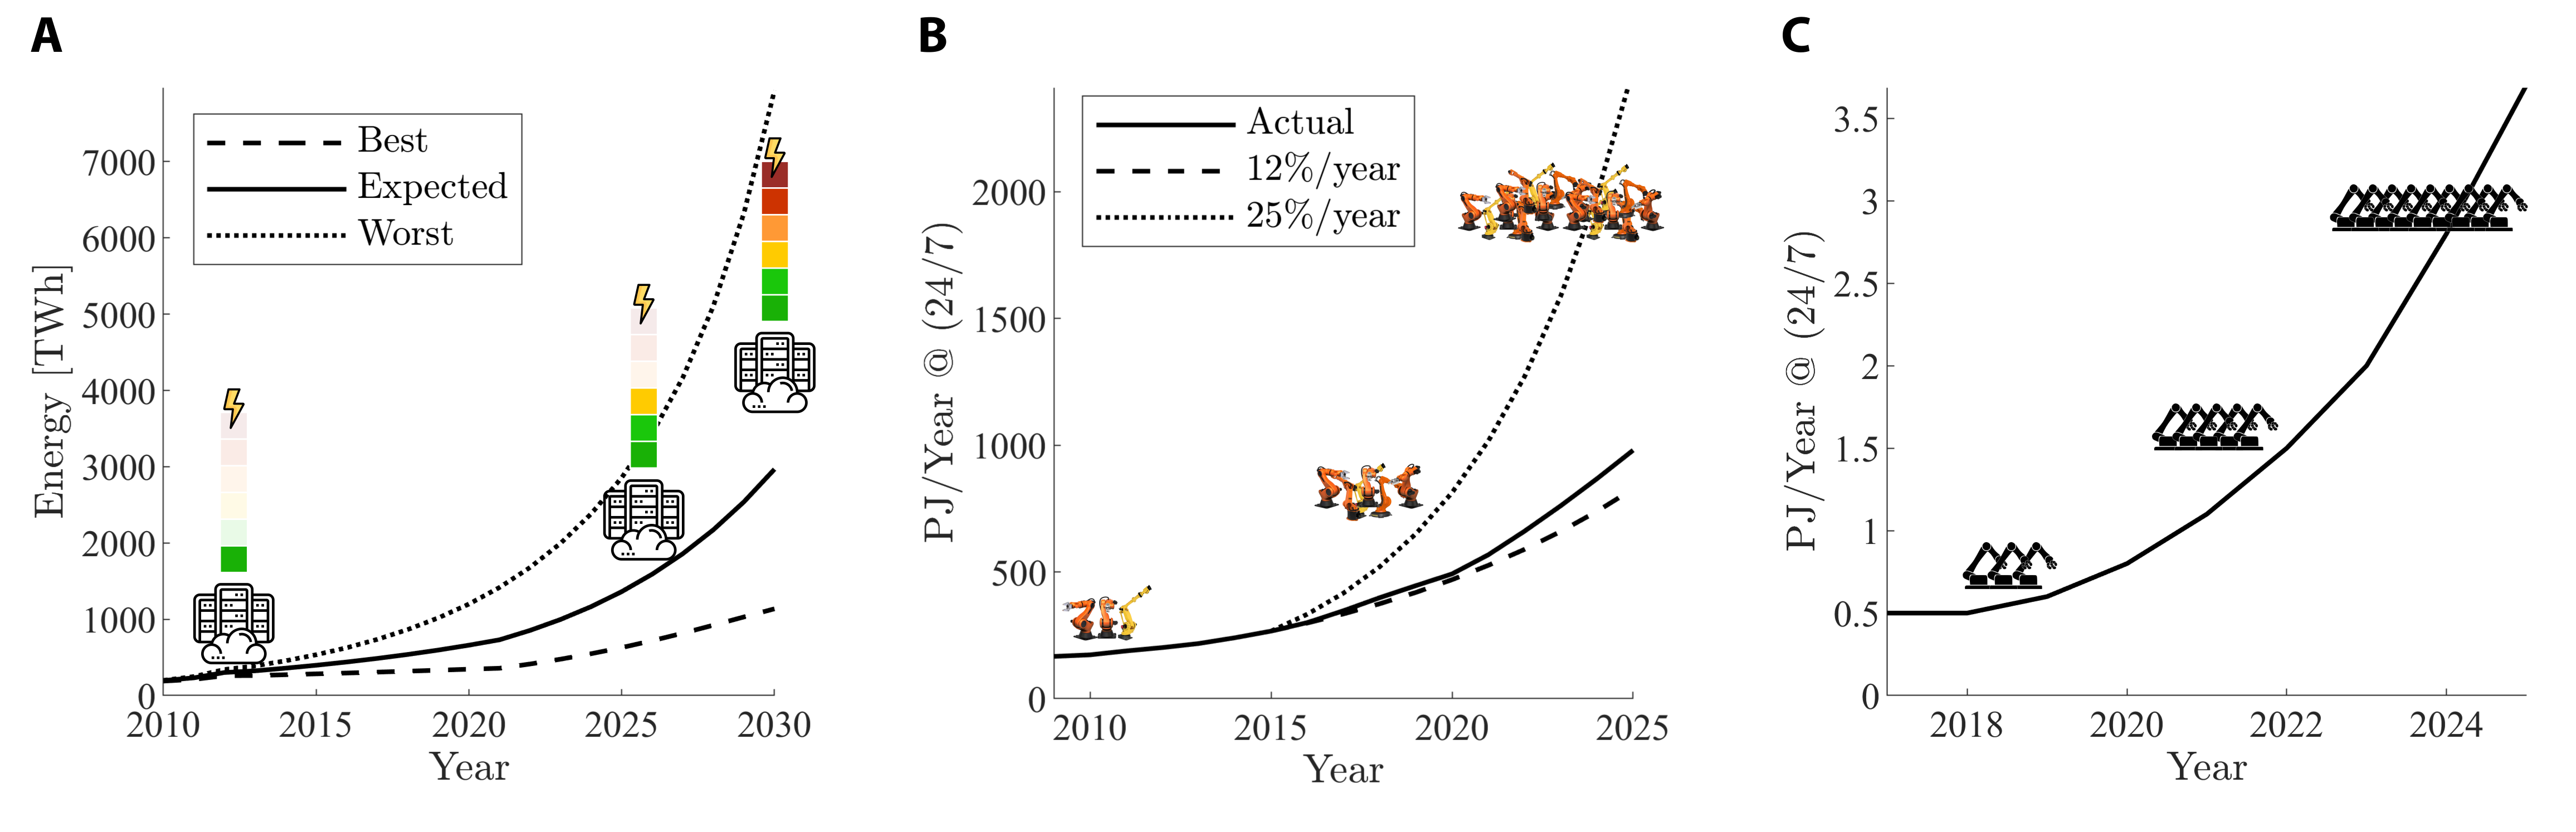
\includegraphics[width=\textwidth]{energy_consumption_trends_ai_and_robotics.png}
	\hspace*{\fill}
	\caption[] {\label{fig:energy_consumption_trends_ai_and_robotics} \textbf{Energy demands in \ac{ai} and robotics.} Global electricity demand of data centers (\textsc{Left}), adapted from \cite{andrae2015global}. The estimated World Robot Energy Consumption of industrial (\textsc{Middle}) and  collaborative robots (\textsc{Right}).}
\end{figure*}
% ---



% ---
\begin{figure*}[t!]
	\centering\section{Materials and Methods}\label{sec:materials_and_methods}
	\hspace*{\fill}
	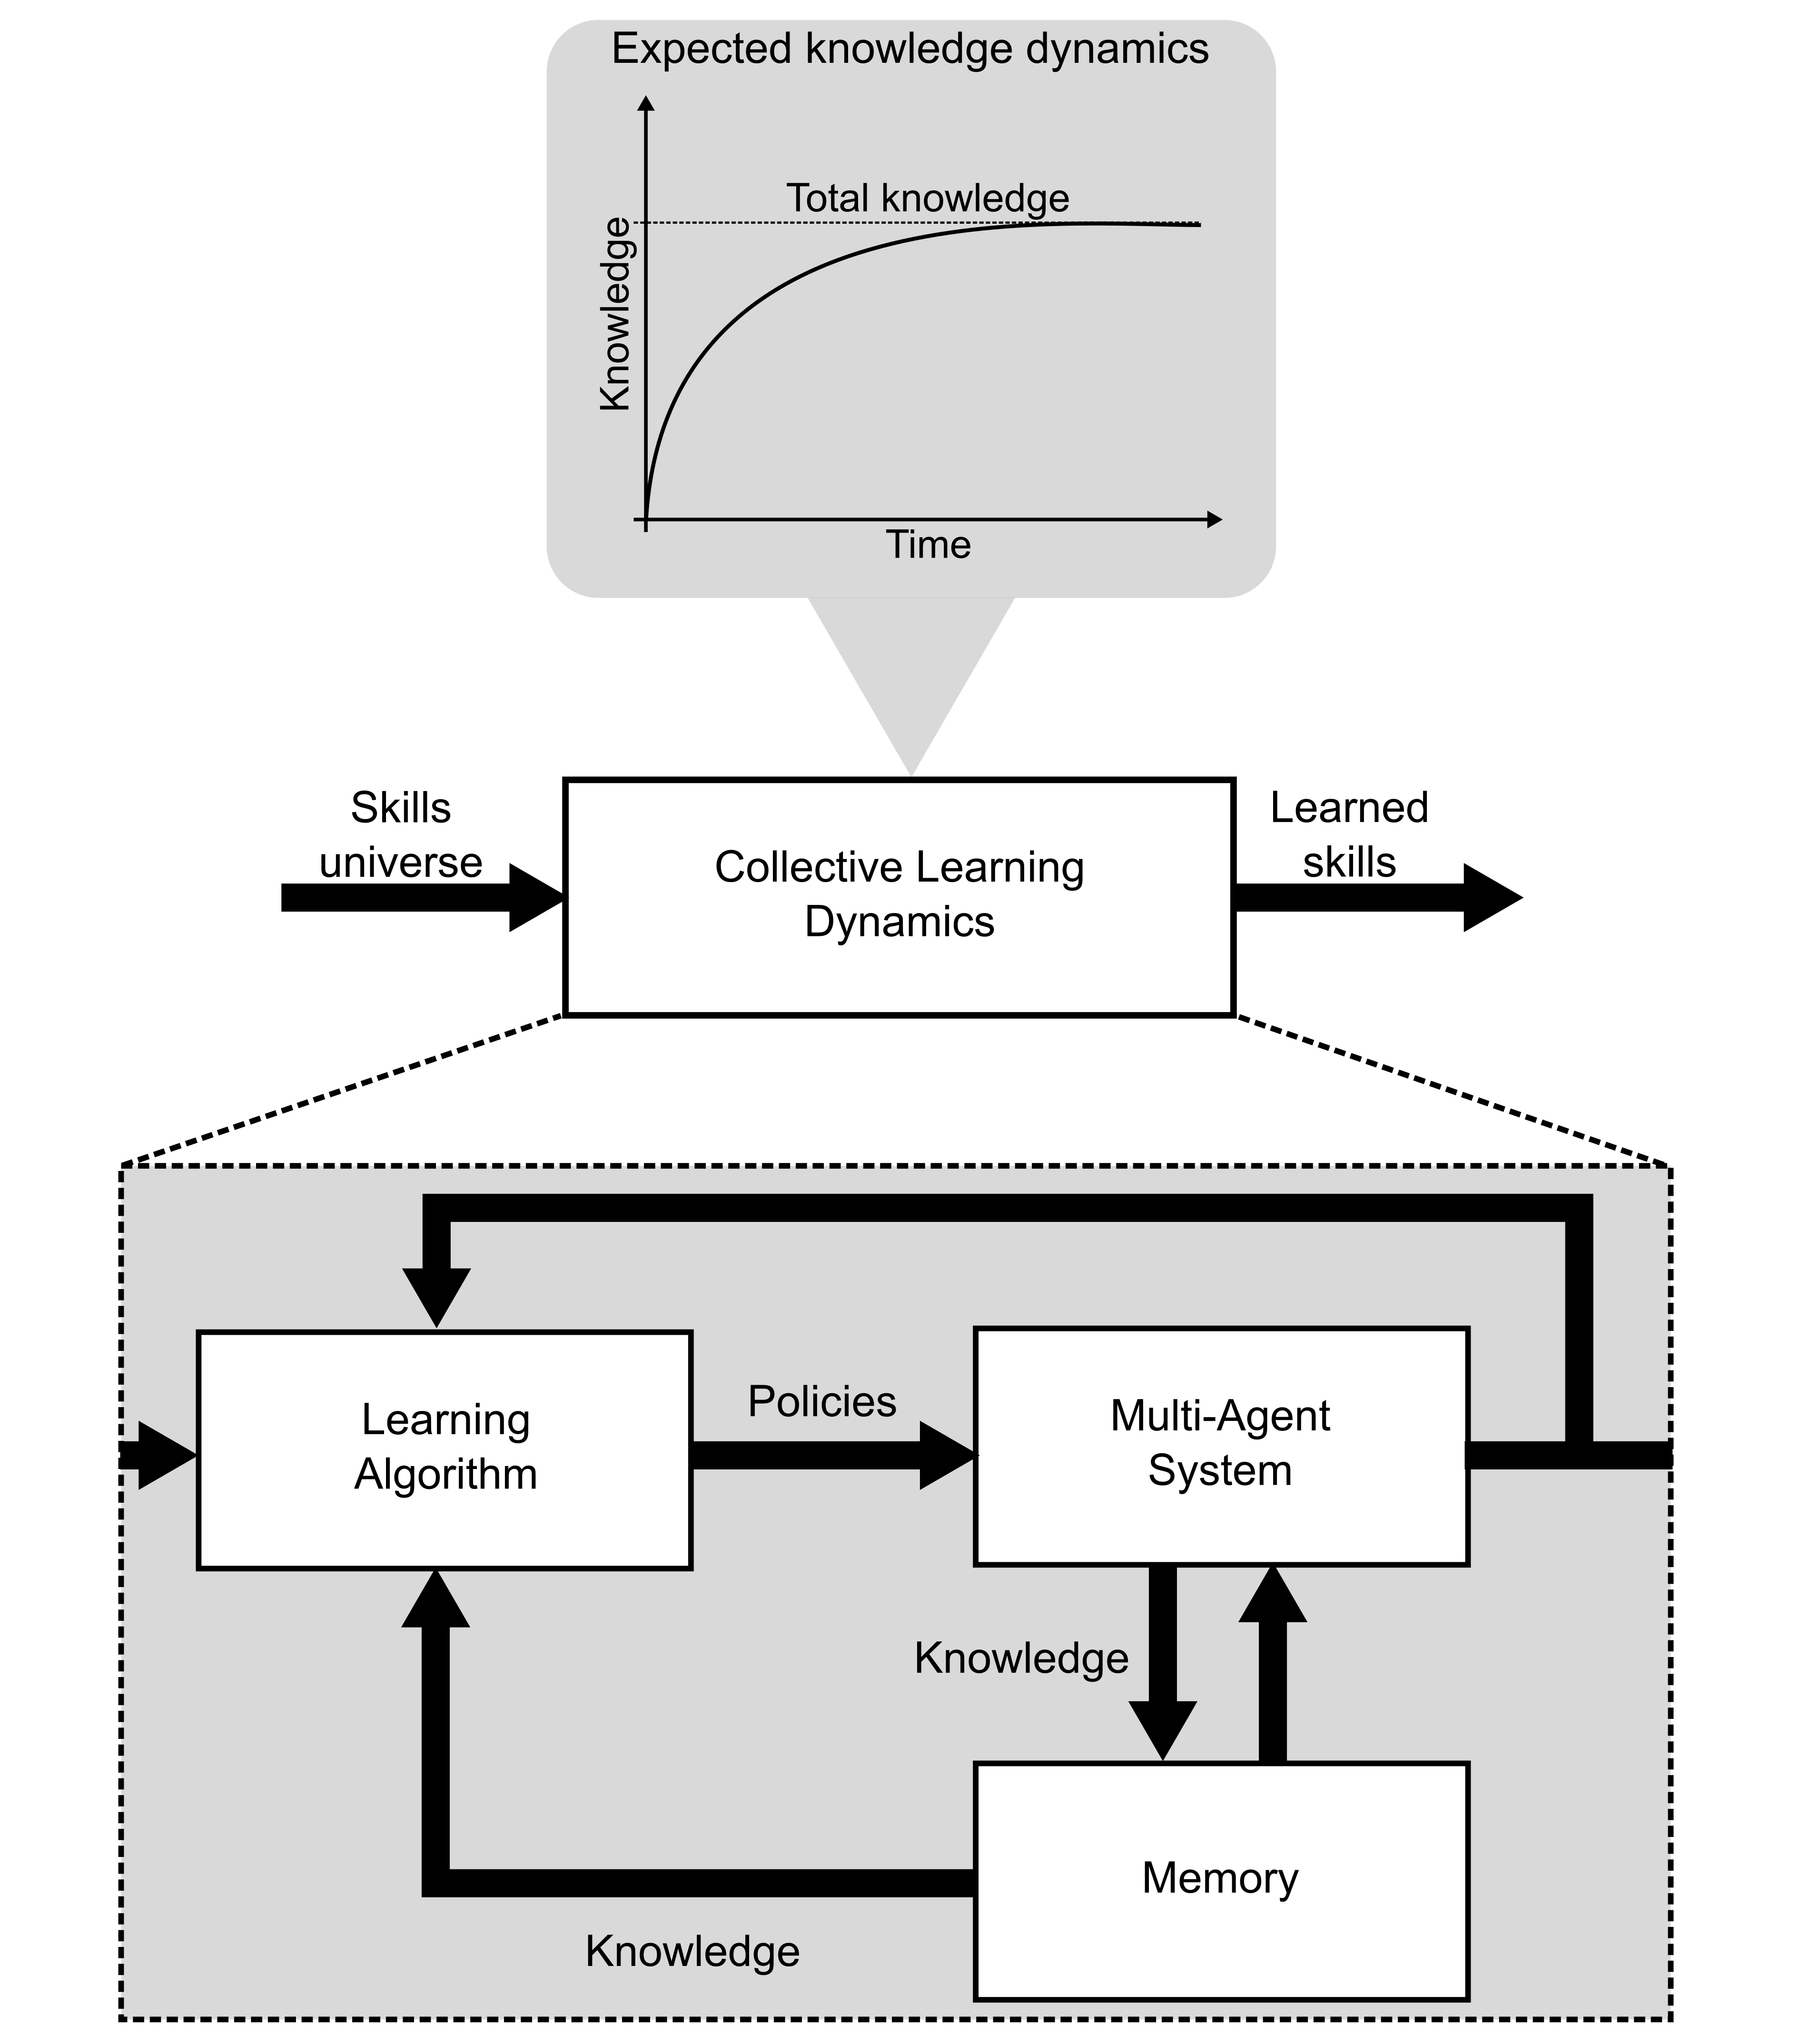
\includegraphics[width=14cm]{closed_loop_collective_dynamics.png}% ===================================================================================================
	\hspace*{\fill}\subsection{Episodic energy and time requirements}\label{sec:power_per_episode}
	\caption[] {\label{fig:collective_learning_system} \textbf{A \acl{cl} system.} {A multi-agent system with appropriate learning algorithm(s) and inter-agent knowledge sharing can learn a universe of skills exponentially fast, as reflected by the exponential collection of the knowledge required to learn the skills.}\pending{Consider sending this figure to the supplementary materials.}}% ---
\end{figure*}\begin{figure}[!h]
% ---	\centering
	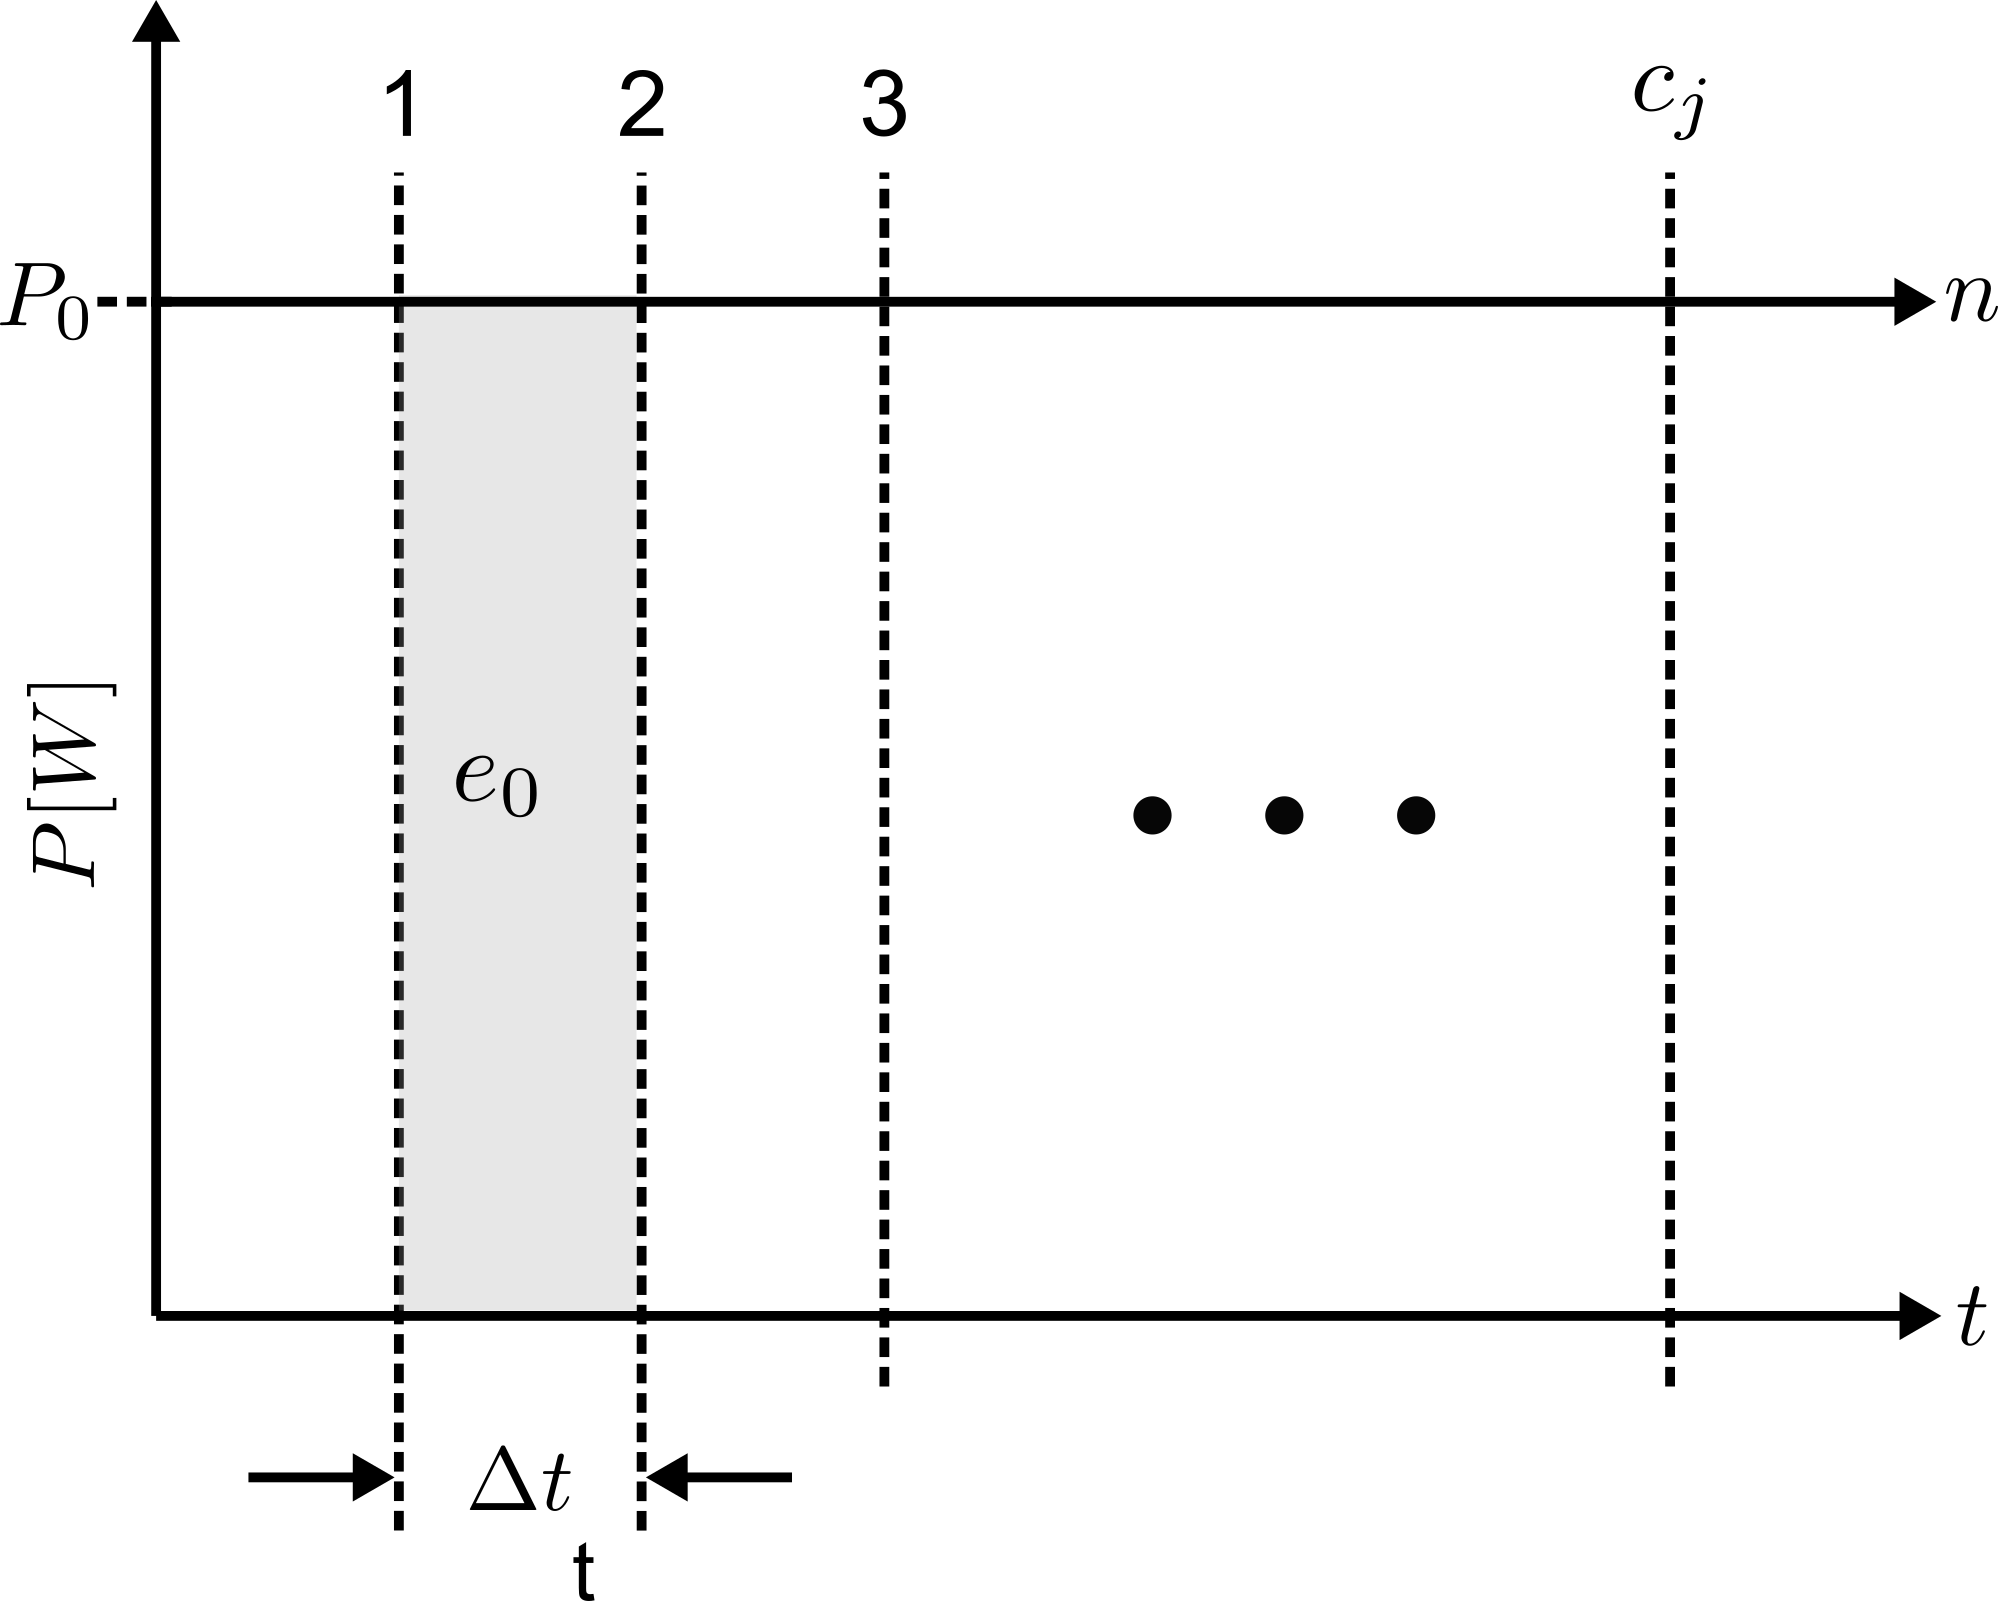
\includegraphics[width=0.45\textwidth]{fig/power_per_episode.png}
	\caption{\textbf{Power consumption per episode.} An episode is an attempt to accomplish a skill. For simplicity, the power to complete an episode is assumed constant.}	
	\label{fig:power_per_episode}
\end{figure}
% ---
\paragraph{Energy requirements.}
Under Asm.~\ref{assumption:power_and_episode_time}, the energy consumption of the $n$-th episode $e_j(n)$ is the constant product
% ---
\begin{equation}\label{eq:energy_per_episode}
	e_j(n) = \underbrace{P_0 \Delta t}_{\text{constant}} = e_0.
\end{equation}
% ---
Consequently, the energy consumed by a robot learning a skill $ s_j $ is directly proportional to the skill complexity $c_j$; i.e.
% ---
\begin{equation}\label{eq:energy_per_skill}
	E_j =\sum_{n=1}^{c_j} e_j(n) = e_0c_j.
\end{equation}
% ---
The energy spent on learning $\mathcal{S}$ under the absence of knowledge sharing is
% ---
\begin{equation}\label{eq:total_energy}
	E_{\mathcal{S}} = \sum_{j=1}^{{N_{\mathcal{S}}}} E_j = e_0 \sum_{j=1}^{{N_{\mathcal{S}}}} c_j%N_{\mathcal{T}} \cdot e_0 \cdot c_j 
\end{equation}
% ---
% ---------------------------------------------------------------------------------------------------
\paragraph{Time requirement.} Similarly, the total learning time $T_{\mathcal{S}}$ for a simple agent is
% ---
\begin{equation}\label{eq:total_time}
	T_{\mathcal{S}} = \Delta t \sum_{j=1}^{{N_{\mathcal{S}}}} c_j.
\end{equation}
% ---

% ===================================================================================================
\subsection{The conventional learning paradigms}\label{sec:types_of_learning}

% ---------------------------------------------------------------------------------------------------
\paragraph{Isolated Learning (IsL)} A robot performs IsL when it learns each skill in $\mathcal{Z}_k$ one after another from the ground up, disregarding the accumulating knowledge from already learned skills. In such a case the rate of convergence and the initial remaining knowledge for all skills are given by
% ---		
\begin{subequations}\label{eq:fg_isolated}
	\begin{alignat}{2}
		f_{j,k}\left(\cdot \right) &=  -\alpha \\
		g_{j,k}\left(\cdot \right) &= 1,
	\end{alignat}
\end{subequations}
% ---
where $ \alpha>0$ models the rate at which a robot in isolation learns any given skill. Relying on Asm.~\ref{assumption:agent_similarity} we can assign a value to $\alpha$ by using the fundamental complexity $c_0$ as follows
% ---
\begin{equation}\label{eq:isolated_learning_rate}
	\alpha = -\frac{1}{c_0}\text{log}(\epsilon).
\end{equation}
% ---
Since in isolated learning $c^{(\text{IsL})}_{j,k} = c_0$, the trial episodes required by one single robot to learn the skills in the cluster $\mathcal{Z}_k$ is given by
% ---
\begin{equation}
	%	\begin{split}
		%		C^{(IsL)}_{k} &= \sum_{j=1}^{N_{\mathcal{Z}}} c^{(IsL)}_{j,k}= N_{\mathcal{Z}}  \cancelto{c_{0}}{c^{(IsL)}_{j,k}} = N_{\mathcal{Z}} c_0
		%	\end{split}
	C^{(\text{IsL})}_{k} = \sum_{j=1}^{N_{\mathcal{Z}}} c^{(\text{IsL})}_{j,k}= N_{\mathcal{Z}}  c^{(\text{IsL})}_{j,k} = N_{\mathcal{Z}} c_0.
\end{equation}
%-- 
Similarly, the total trial episodes to learn the universe of skills is simply
% ---
\begin{equation}
	C^{(\text{IsL})}_{\mathcal{S}} = N_\mathcal{K} N_{\mathcal{Z}} c_0.
\end{equation}
% ---

\textbf{Multi agent case.} Suppose that a batch of $m$ robots is used to learn the same number of skills in parallel in a given cluster $\mathcal{Z}_k$. Such a strategy only distributes equally the total number of episodes by the number of available robots; i.e.
% ---
\begin{equation}
	^{\lvert \lvert}C^{(\text{IsL})}_k=  \overbrace{\frac{1}{m}C^{(\text{IsL})}_k}^{\text{episodes per robot}}.
\end{equation}
% ---

% ---------------------------------------------------------------------------------------------------
\paragraph{\textbf{Incremental Learning (IL)}}
It corresponds to the continuous aggregation and exchange of knowledge from \emph{intra-cluster} skills. Referring back to Asm.~\ref{assumption:skill_clustering}, the knowledge from skills belonging to a cluster ${\mathcal{Z}_k}$ can be be leveraged by an agent in virtue of their significant similarity. As depicted in Fig.~\ref{fig:intra_skill_learning}, a robot ($r_1$ in this case) learns every skill in $\mathcal{Z}_1$ with a rate $\alpha$---the self loops---but also retains and uses the acquired knowledge to learn subsequent skills. The effect of incremental learning on the knowledge collection rate can be modeled to be directly proportional to the number of learned skills as
% ---
\begin{equation}\label{eq:f_function_incremental}
	f_{j,k}\left(N_{\zeta_k}\right) = -\alpha\left(\eta N_{\zeta_k} + 1 \right), 
\end{equation}
% ---
where $\eta>0$ represents the efficiency of knowledge exchange from $\zeta_k$ to $s_{j,k}$. Different potential models might be used to model the depletion of the initial remaining knowledge represented by $g_{j,k}\left(N_{\zeta_k}\right)$, e.g. a linear decay rate, our expectation is that, under the assumption that a learning strategy involving the ordering of skills according to similarity and their balanced distribution in the different clusters, $g_{j,k}\left(N_{\zeta_k}\right)$ might naturally resemble an exponential decay that is strongly dependent on $N_{\zeta_k}$. Such considerations motivate our choice of the following function
% ---
\begin{equation}\label{eq:g_function_incremental}
	g_{j,k}\left(N_{\zeta_k}\right) = e^{-\delta N_{\zeta_k}},
\end{equation}
%---
again with a factor $\delta>0$ controlling the rate at which the exponential converges. Similar to $\alpha$, using Asm.~\ref{assumption:cluster_size} $\delta$ can be defined as 
% ---
\begin{equation}\label{eq:delta}
	\delta = -\frac{1}{N_\mathcal{Z}}\text{log}(\epsilon).
\end{equation}
% ---
Essentially, such choice of $\delta$ implies that the remaining knowledge in a cluster after seeing all its skills is negligible. Via the exchange factors $(\eta,\delta)$, in incremental learning the knowledge about every new skill gets gradually increased by leveraging previous knowledge, resulting in
% ---
\begin{equation*}\label{eq:remaining_knowledge__IL}
	\bar{\sigma}^{(\text{IL})}_{i,j}(n) = e^{-\alpha  \left(\eta N_{\zeta_k}+1\right) n} e^{-\delta N_{\zeta_k}}.
\end{equation*}
% ---
As the complexity $c_{j,k}$ of a skill can also be interpreted as the number of trial episodes required for the remaining knowledge to go below a threshold $\epsilon$; i.e.
% ---
\begin{equation*}
	\bar{\sigma}^{(\text{IL})}_{i,j}(n) \Big \rvert_{n \ge c^{(\text{IL})}_{j,k}} \leq \epsilon.
\end{equation*}
% ---
Then, under this scheme the complexity $c^{(\text{IL})}_{j,k}$ to learn a new is skill in the cluster results in
% ---
\begin{equation}\label{eq:complexity_IL}
	c^{(\text{IL})}_{j,k} = -\frac{\text{log}(\epsilon) - \text{log}\left(\bar{\sigma}^{(IL)}_{j,k}(0)\right)}{\alpha (\eta N_{\zeta_k}+ 1)} = -\frac{\text{log}(\epsilon) + \delta N_{\zeta_k}}{\alpha (\eta N_{\zeta_k}+ 1)}  .
\end{equation}
% ---
The total number of trial episodes $ C_k $ that an agent following an incremental learning strategy needs to learn the $N_{\mathcal{Z}_k}$ skills in a cluster $ \mathcal{Z}_k $ is given by
% ---
\begin{align}\label{eq:total_episodes_incremental}
	\begin{split}
		C^{(\text{IL})}_k &= \sum^{N_{\mathcal{Z}}}_{j=1} c^{(\text{IL})}_{j,k}.
	\end{split}
\end{align}
% ---

\textbf{Multi-agent case.} If $m$ robots are used in parallel to divide the load of learning the tasks then
% ---
\begin{align}
	\begin{split}
		{}^{\lvert \rvert}C^{(IL)}_k &= \sum^{\frac{N_{\mathcal{Z}}}{m}}_{j=1} c^{(IL)}_{j,k}.
	\end{split}
\end{align}
% --
In essence, using $m$ robots without exchanging knowledge only subdivides the learning in every cluster into $m$ smaller problems \emph{without adding any additional benefit to the rate at which knowledge is acquired}. 

% ---------------------------------------------------------------------------------------------------
\paragraph{\textbf{Transfer + Incremental Learning (TIL)}}
Transfer learning (TL) alone refers to the one-time \emph{inter-cluster} exchange of knowledge. Considering $\mathcal{K} = \{ \mathcal{Z}_k \}^{N_\mathcal{K}}_{k=1}$ to be the set of all available skill clusters, TL represents the exchange of knowledge from the skills learned in different \emph{origin} clusters $\mathcal{O} = \{ \mathcal{Z}_1,\mathcal{Z}_2,\ldots,\mathcal{Z}_{k-1} \}$ to the skills that will be learned in a \emph{destination} cluster $\mathcal{Z}_k$ (see Fig.~\ref{fig:cluster_to_cluster_knowledge_transfer_parallel}). Concretely, the effect that TL has on the skills of the destination cluster is the reduction of the initial remaining knowledge and the increase of the initial learning rate for all the skills in the $k$-th cluster via the parameter $\beta_k$; i.e.
% ---
\begin{equation}\label{eq:f_function_transfer}
	f_{j,k}\left(N_{\zeta_k}\right) = -\alpha \left( \frac{\eta N_{\zeta_k} + 1}{1 - \beta_k} \right),
\end{equation}
% ---
and
% ---
\begin{equation}\label{eq:g_function_transfer}
	g_{j,k}\left(N_{\zeta_k}\right) = (1-\beta_k) e^{-\delta N_{\zeta_k}}.
\end{equation}
%---
In essence, $\beta_k$ is the head start granted by knowledge transfer from other clusters to the skills in $\mathcal{Z}_k$. We argue that  $0<\beta_{k} < 1$ since it represents the \emph{aggregated} knowledge exchange factor from the different origin clusters $\mathcal{Z}_{c}$ to the target cluster $\mathcal{Z}_{k}$. Let $0<\beta_{c} < 1$ be the transfer contribution factor of a single origin cluster $\mathcal{Z}_c$. Additionally, consider that
% ---
\begin{equation}
	\sum\limits_{c=1}^{N_\mathcal{K}}\beta_{c} \leq 1,
\end{equation}
% --
as $1$ represents all the knowledge in $\mathcal{S}$. Asm.~\ref{assumption:cluster_transferability} implies that $\beta_c$ is equal for all the clusters. In this work we select $\beta_c = 1/N_\mathcal{K}$ for simplicity. The aggregated transfer factor $\beta_k$ is the sum of the individual factors from the already-visited clusters; i.e.
% ---
\begin{equation}\label{eq:beta_k_transfer}
	\beta_{k}= \left(k-1\right)\beta_c = \left(k-1\right)\frac{1}{N_\mathcal{K}}.
\end{equation}
% ---

Consequently, the remaining knowledge when transfer and incremental learning are used in conjunction is
% ---
\begin{equation}\label{eq:remaining_knowledge__ITL}
	\bar{\sigma}^{(\text{TIL})}_{j,k}(n) = \left(1- \beta_k\right) e^{-\alpha  \left(\frac{ \eta N_{\zeta_k}+1}{1 - \beta_k}\right) n} e^{-\delta N_{\zeta_k}}.
\end{equation}
% ---
Similar to incremental learning, the complexity to learn a skill in transfer learning is
\begin{equation}\label{eq:skill_complexity_TL}
	c^{(\text{TIL})}_{j,k} = -\frac{1 - \beta_{k}}{\alpha (\eta N_{\zeta_k}+ 1)}\left[\text{log}(\epsilon) + \delta N_{\zeta_k} - \text{log}(1 - \beta_{k})\right]
\end{equation}
% ---
and the total number of episodes  $ C_k $ that an agent requires to learn the $N_{\mathcal{Z}_k}$ skills is merely their sum
% ---
\begin{align}\label{eq:total_episodes_transfer}
	\begin{split}
		C^{(\text{TIL})}_k &= \sum^{N_{\mathcal{Z}}}_{j=1} c^{(\text{TIL})}_{j,k}.
	\end{split}
\end{align}
% --- 

\textbf{Multi-agent case.} If $m$ robots are used in parallel to divide the load of learning the tasks then, the transfer of knowledge from cluster to cluster is also divided by the number of robots, this implies that \eqref{eq:beta_k_transfer} changes to
% ---
\begin{equation}\label{eq:beta_k_transfer_parallel}
	{}^{\lvert \rvert}\beta_{k}= \frac{1}{m}\beta_{k}.
\end{equation}
% ---
Correspondingly, when using transfer learning in parallel $\beta_k$ is replaced by ${}^{\lvert \rvert}\beta_{k}$ in \eqref{eq:skill_complexity_TL}. Then, similar to IL, the total number of episodes to learn the skills in a cluster is
% ---
\begin{align}
	\begin{split}
		{}^{\lvert \rvert}C^{(\text{TIL})}_k &= \sum^{\frac{N_{\mathcal{Z}}}{m}}_{j=1} c^{(\text{TIL})}_{j,k}.
	\end{split}
\end{align}
% ---
This case is depicted on Fig.~\ref{fig:cluster_to_cluster_knowledge_transfer_parallel}, where two robots $ r_1$ and $r_2$ learn skills in four different clusters. The shaded areas are the subclusters of skills learned by each robot. Since they do not share knowledge between them, each robot has access only to the knowledge it has collected and cannot benefit from one another. 

% ---------------------------------------------------------------------------------------------------
%\subsection*{\textbf{Collective learning (CL)}}
%As mentioned in Sec.~\ref{sec:intro}, EAI agents will be a core element of industrial, healthcare, and domestic ecosystems with advanced communication and remote processing capabilities. Given the anticipated legions of EAI agents executing and learning several different skills at any given time in those environments, it is immediately evident that the previous learning paradigms are not meant to exploit these large number of agents together with the advanced communication and processing infrastructure to take full advantage of the potential for concurrent knowledge exchange among the agents. Therefore, the use of isolated, incremental, and transfer learning by these many agents 
%would directly aggravate computational demand (see challenge C1). As discussed in \cite{Kaelbling2020foundationefficientrobot} an leaning algorithm that would allow an agent to learn new tasks on-the-fly would need to be sample-efficient, generalizable, compositional, and (truly) incremental. Collective learning is the natural paradigm that meets this requirements exploiting the full communication potential of the networked EAI agents to leverage the real-time synergistic exchange and aggregation of collected knowledge to make the learning of tasks energy- and time-efficient.
%
%To formalize this idea, let $ \left\lbrace \rho_i \right\rbrace_{i=1}^{m} $ be a set of robotic agents that defines a community of robots. In collective learning, the different robotic agents $ \rho_i $ develop and accumulate dynamically a common mind (body of knowledge) via networked interactions where individual experience, knowledge and skills are disseminated to all the other elements in the collective. Information flows vertically as previous knowledge is passed on, as well as horizontally by sharing concurrent experience between agents. Via these mechanisms, knowledge can be replicated, complimented and further developed. We take from \cite{Garavan2012CollectiveLearning} two notions central in collective learning that are applicable to the embodied AI agents:
%% ---
%\begin{enumerate}
%	\item Capability to restructure and meet changing conditions
%	\item Aggregation of skills, knowledge, and behaviors
%\end{enumerate}
%% ---
%Collective learning contrasts with the previously discussed incremental learning in that a single agent $ r_i $ can aggregate only so much knowledge via trial and error and is limited by a sequential learning structure. Learning collectively, on the other hand, enforces parallelization of knowledge acquisition via the concurrent learning and sharing of all agents as they acquire new skills, knowledge. Moreover, collective learning involves not only the information acquisition, but also how this information is brought to use to form and develop knowledge. 
%
%CL is not only a promising research direction but, in our opinion, has the potential to be a unifying solution to the grand challenges posed by embodied AI. Furthermore, by incorporating new mechanical designs as elements of the learning pipeline it is possible to iteratively evaluate the energy efficiency of proposed solutions and select the best ones as reference designs for future manufacturing processes with underlying learning, therefore, promoting a cyclical optimization towards a semi-optimal general design.
%
%Unlike isolated and transfer learning, in this paradigm a batch of robots $\left \lbrace r_i \right \rbrace^m_{1}$ not only learn different skills concurrently but also exchange the acquired knowledge between each other and are actually able to leverage it. To enable CL, it is assumed that
%\begin{itemize}
%	\item an inter-agent communication protocol/infrastructure is in place that
%	\item enables agents to concurrently exchange and integrate the self-acquired and received knowledge to
%	\item incrementally speed up the learning of all the agents as a whole.
%\end{itemize}
%% ---
%As a result, the intra- and inter-cluster knowledge transfer is possible. Naturally, the CL paradigm involves a complex scheduling problem to determine the optimal skill distribution and inter-agent knowledge sharing strategy. Since we have not tackled this problem yet, we ground the subsequent discussion on Assumptions~\ref{assumption:average_behavior}, \ref{assumption:agent_similarity},~\ref{assumption:cluster_size}, and~\ref{assumption:cluster_transferability} that suggest an average behavior given a suitable scheduling.
%
%Fig.~\ref{fig:cl_example_figure} illustrates the CL concept, where the self loop represents the dynamics of a single robot learning (at a rate $\alpha$). The exchange of knowledge across agents is represented via the cross-couplings weighted by a parameter $\gamma$ that models how efficient is the bidirectional pairwise knowledge exchange. Similar to transfer learning, if two robots exchange knowledge about skills with low similarity (i.e. skills in different clusters), then $\gamma$ is scaled by the inter-cluster transferability parameter $\beta$. In CL \eqref{eq:simple_knowledge_dynamics} is extended to 
%% ---
%\begin{subequations}\label{eq:collective_knowledge_dynamics}
%	\begin{empheq}[left=\empheqlbrace]{align}
%		\dot{\bar{\bm{\sigma}}}^{(CL)}_{j,k}\left(n\right) &= \left[  f_{j,k}\left(N_{\zeta_k},r\right) \bm{I} + \gamma \bm{A} \odot \bm{B}  \right] \bar{\bm{\sigma}}^{(CL)}_{j,k}\left(n\right)\\
%		\bar{\bm{\sigma}}^{(CL)}_{j,k}(0) &= g_{j,k}\left( N_{\zeta_k}, r\right) \bm{I},
%	\end{empheq}
%\end{subequations}
%% ---
%where $r=m$ is the number of robots that exchange knowledge among them. This implies that now $\bar{\bm{\sigma}}^{}_{j,k} \in \mathbb{R}^r$ is a vector that represents the dynamics of the remaining knowledge of all the $m$ skills being concurrently learned. $\bm{A} \in \mathbb{R}^{r \times r}$ is a zero-diagonal symmetric adjacency matrix whose entry $(\bm{A})_{i,j} = 1$ if robot $i$ exchanges knowledge with robot $j$ and $(\bm{A})_{i,j} = 0$ if it does not. The term $\gamma \in \mathbb{R}_+ $ weighs the knowledge exchange strength among robots. Furthermore, since there may be robots learning skills in different clusters at the same time, the matrix $\bm{B}$, whose entries are $\left(\bm{B}\right)_{i,j} \in \left \lbrace 1, \beta_{k} \right \rbrace$, with
%% ---
%\begin{equation}
%	%\beta_{k} = 1/N_\mathcal{K}, 
%	\beta_{k} = r\frac{ N_{\zeta_k}}{N_\mathcal{S}}, 
%\end{equation}
%% ---
%scales down the knowledge contributions between robots from different clusters. Finally, the operator $\odot$ represents the Hadamard product of matrices. The functions $ f(\cdot)$ and $g(\cdot)$ are now also dependent on the number of robots that exchange knowledge, which directly impacts the number of skills that enter $\zeta_k$ after a learning cycle; i.e.
%% ---
%\begin{equation}\label{eq:f_function_collective}
%	f_{j,k}\left(N_{\zeta_k},r\right) = -\alpha \left( \frac{\eta r N_{\zeta_k} + 1}{1 - \beta_k} \right),
%\end{equation}
%% ---
%and
%% ---
%\begin{equation}\label{eq:g_function_collective}
%	g_{j,k}\left(N_{\zeta_k},r\right) = (1-\beta_k) e^{-\delta r N_{\zeta_k}}.
%\end{equation}
%%---
%Some considerations need to be taken when selecting the value of $\gamma$ given that the dynamics matrix of the collective system
%% ---
%\begin{equation}
%	\bar{\bm{A}}\left(N_{\zeta_k}\right) = f\left(N_{\zeta_k},r\right) \bm{I} + \gamma \bm{A} \odot \bm{B} 
%\end{equation} 
%% ---
%exhibits a dependency on the number of seen skills $N_{\zeta_k}$, which is directly influenced by the number of robots $r$ in the collective. Yet, it can be proven that there is a coupling strength $\gamma$ for a given connectivity $\bm{A}$ that ensures that the remaining knowledge for all skills converges asymptotically to zero.

% ===================================================================================================
%                                                 |                                                 |
%                                                 |                                                 |
% -------------------------------------------- SECTION ---------------------------------------------|
%                                                 |                                                 |
%                                                 |                                                 |
% ===================================================================================================
% ===================================================================================================
\newpage
\section{Analysis of the collective learning behavior}\label{sec:collective_learning_analysis}

\textcolor{blue}{\textbf{THIS TEXT GOES TO SUPPLEMENTARY IN THE STABILITY ANALYSIS}} where the operator $\odot$ represents the Hadamard product of matrices. This expression models $r=m$ robots exchanging knowledge among each other. The vector $\bar{\bm{\sigma}}^{}_{j,k} \in \mathbb{R}^r$ represents the dynamics of the remaining knowledge of all the $m$ skills being concurrently learned. $\bm{A} \in \mathbb{R}^{r \times r}$ is a zero-diagonal symmetric adjacency matrix whose entry $(\bm{A})_{i,j} = 1$ if robot $r_i$ exchanges knowledge with robot $r_j$ and $(\bm{A})_{i,j} = 0$ if it does not.

$\ldots$ the matrix $\bm{B}$, whose entries are $\left(\bm{B}\right)_{i,j} \in \left \lbrace 1, \beta_{k} \right \rbrace$, $\ldots$

% ===================================================================================================
%                                                 |                                                 |
%                                                 |                                                 |
% -------------------------------------------- SECTION ---------------------------------------------|
%                                                 |                                                 |
%                                                 |                                                 |
% ===================================================================================================

\section{Results}\label{sec:use_case_results}
Fig.~\ref{fig:collective_learning} shows the results of applying isolated learning, incremental learning, transfer and incremental learning, and collective learning to the learning scenario defined by the tuple
% ---
\begin{equation*}
	\phi_{SF} = \left(N_\mathcal{S}= 512, N_\mathcal{K}=4, m=32, \left[\alpha =  0.0461, \delta =  0.0360, \eta= 0.1\right]\right).
\end{equation*}
% ---
In this scenario all $m$ agents are always concurrently learning skills from the same cluster $Z_i$.
% ---
\begin{figure}[!h]
	\centering
	\hspace*{\fill}
	\subfloat[]{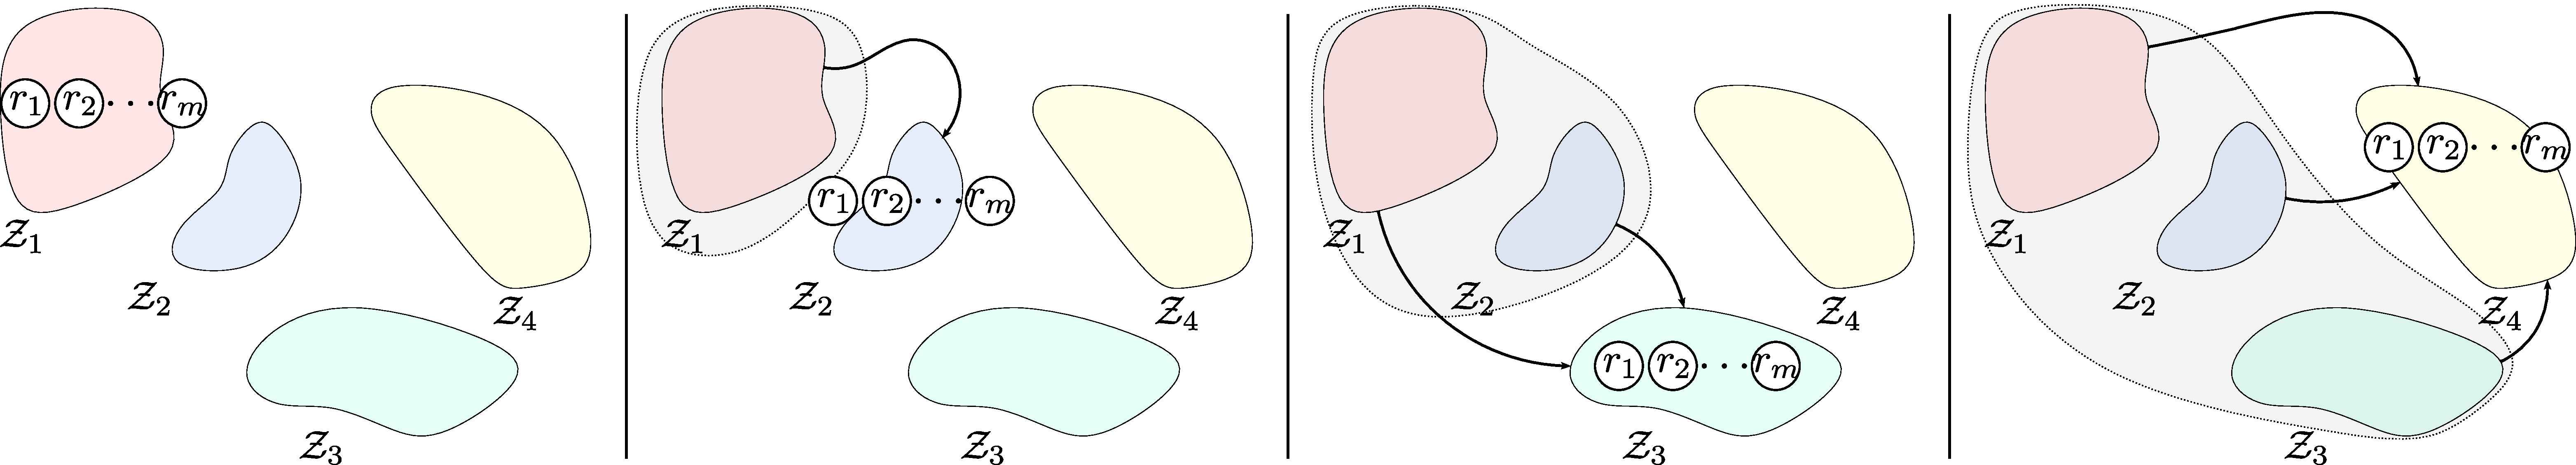
\includegraphics[width= 0.7\textwidth]{fig/cluster_learning_sequence.png} \label{fig:cluster_learning_sequence}}
	\hspace*{\fill}
	\\	
	\hspace*{\fill}
	\subfloat[]{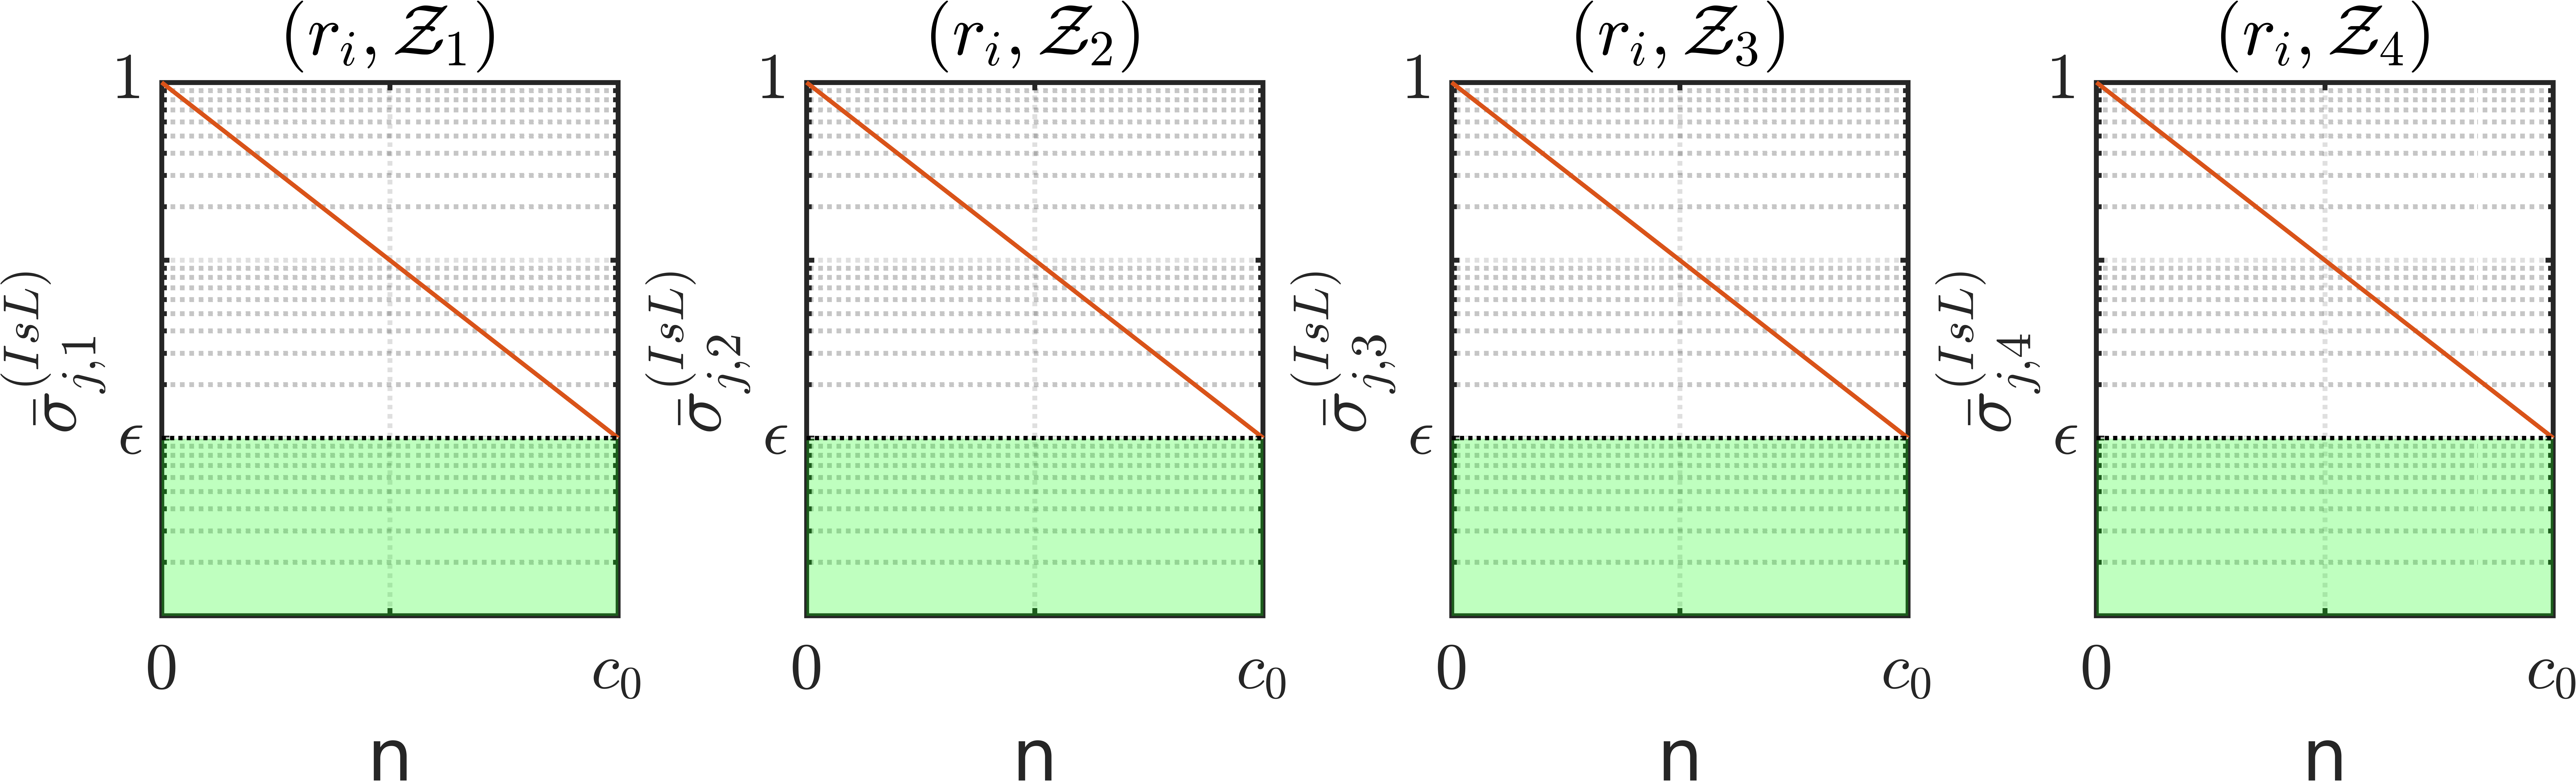
\includegraphics[width= 0.7\textwidth]{fig/dynamics_isolated_learning.png} \label{fig:dynamics_isolated_learning}}  
	\hspace*{\fill}
	\\	
	\hspace*{\fill}
	\subfloat[]{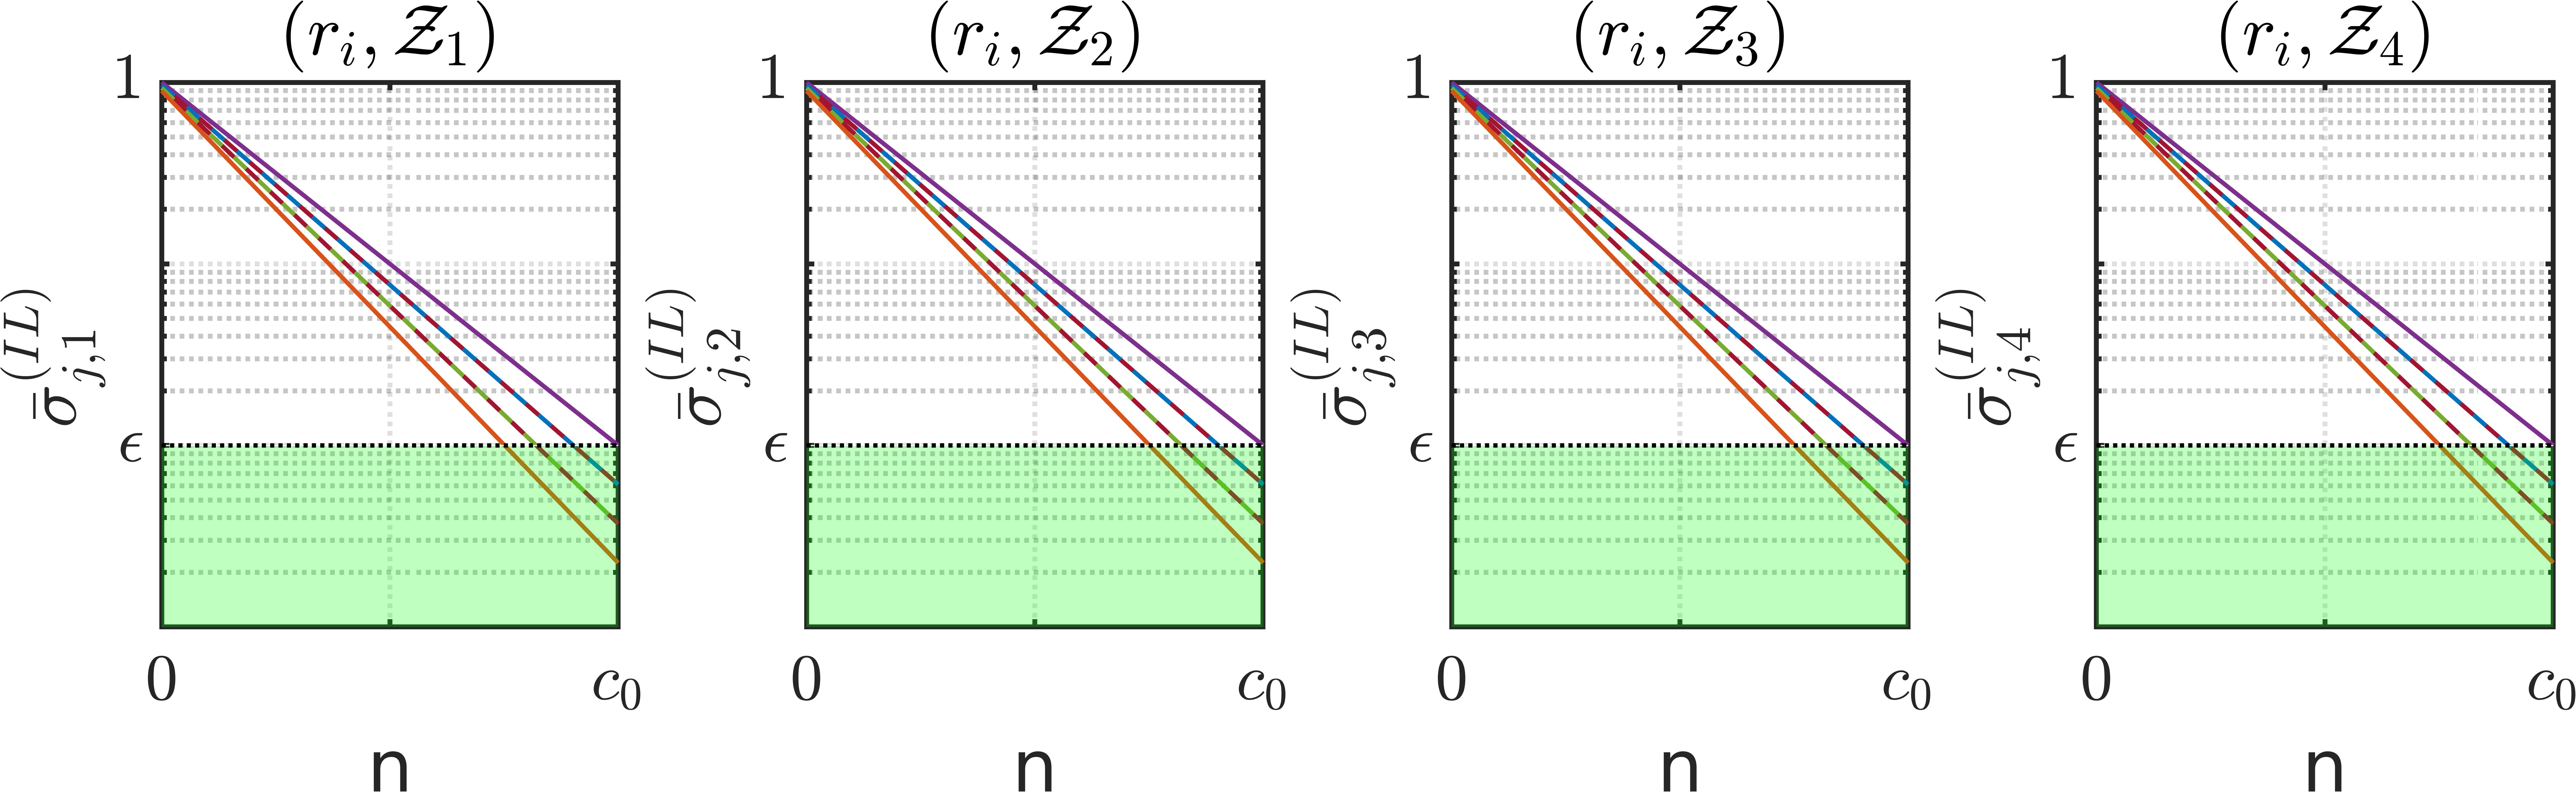
\includegraphics[width= 0.7\textwidth]{fig/dynamics_incremental_learning.png} \label{fig:dynamics_incremental_learning}}  
	\hspace*{\fill}	
	\\
	\hspace*{\fill}
	\subfloat[]{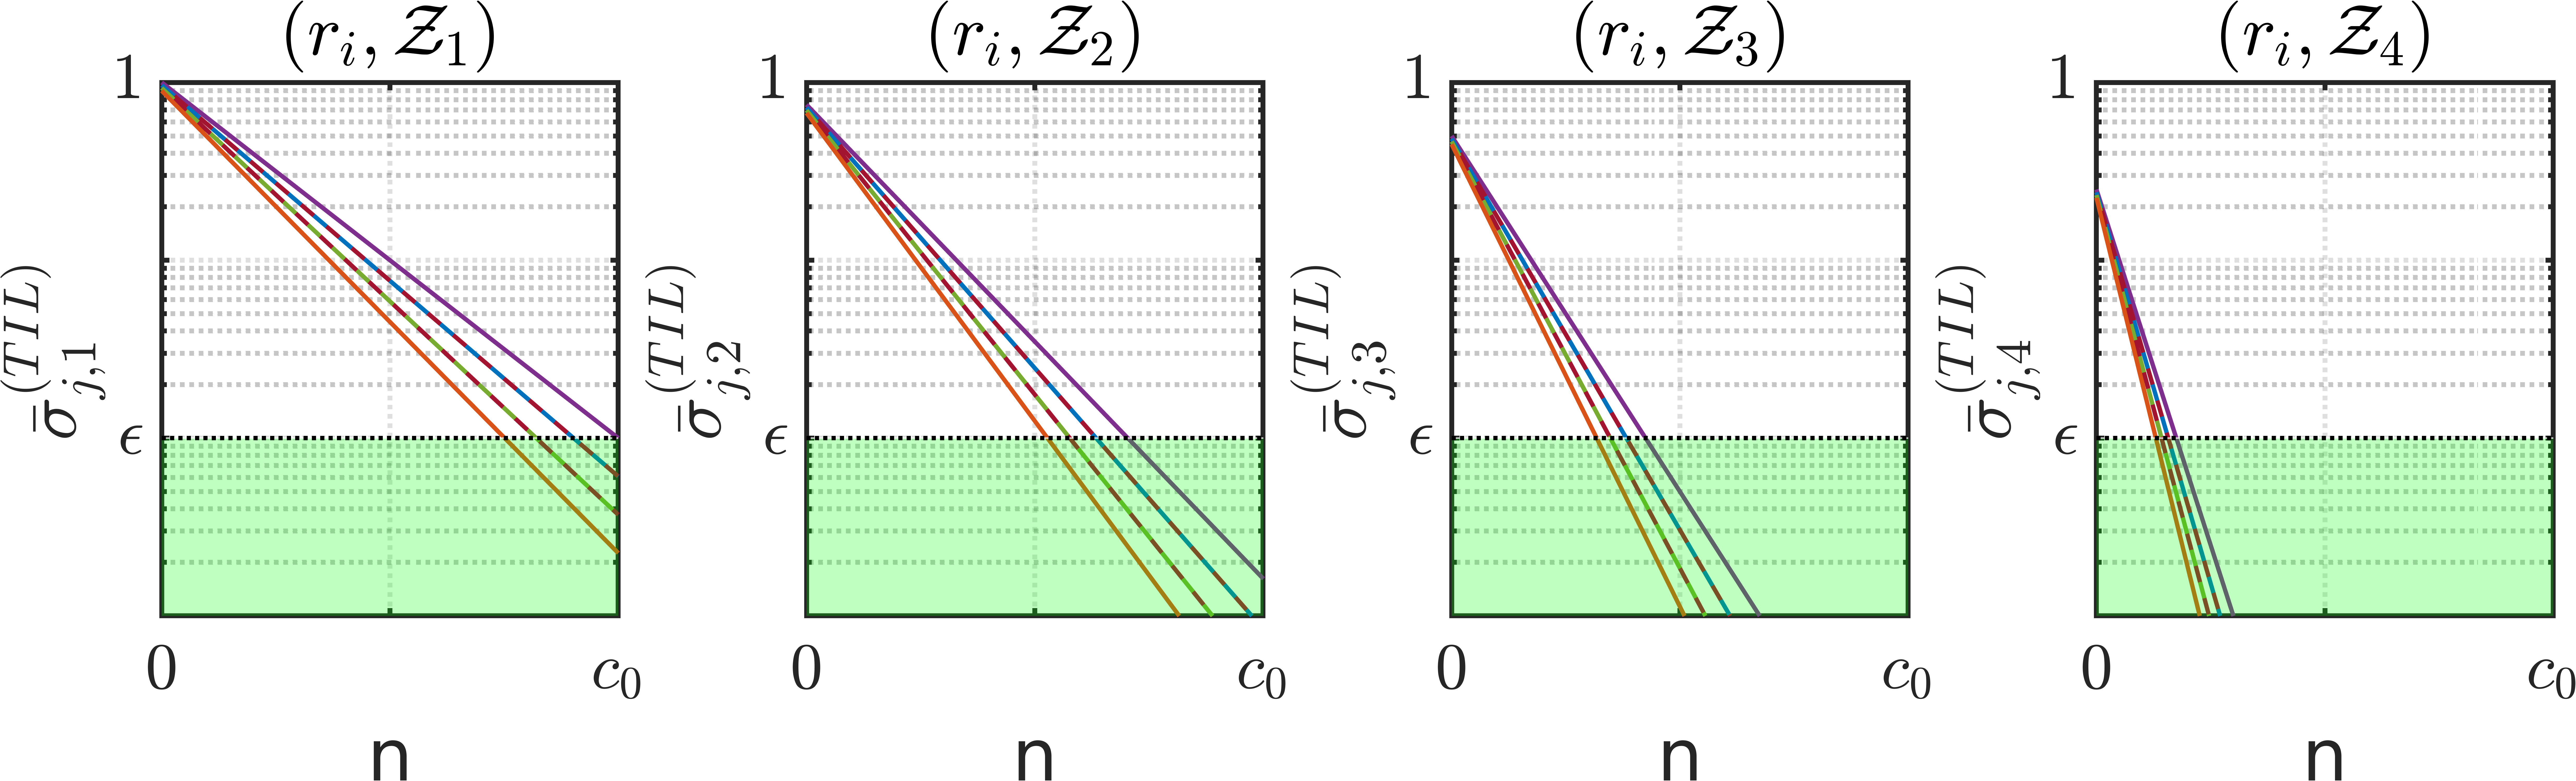
\includegraphics[width= 0.7\textwidth]{fig/dynamics_incremental_transfer_learning.png} \label{fig:dynamics_incremental_transfer_learning}}  
	\hspace*{\fill}
	\\
	\hspace*{\fill}
	\subfloat[]{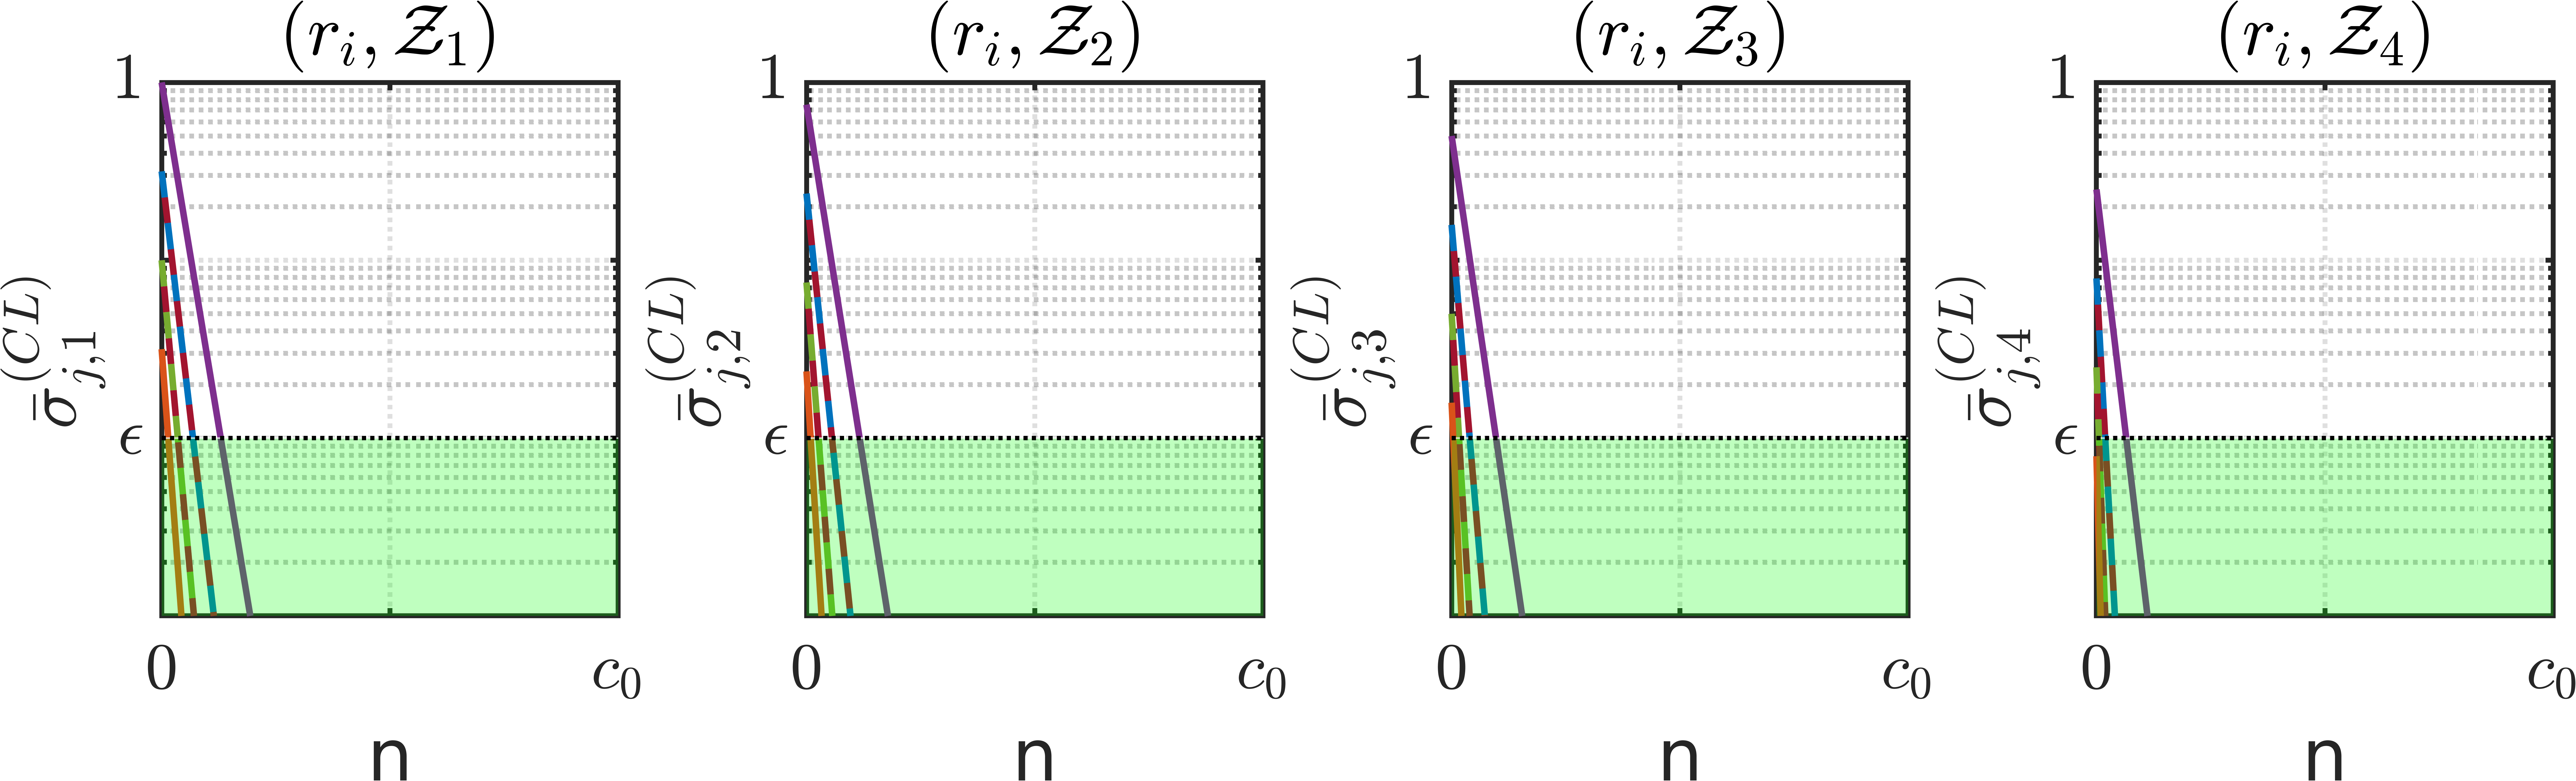
\includegraphics[width= 0.7\textwidth]{fig/dynamics_collective_learning.png} \label{fig:dynamics_collective_learning}}
	\hspace*{\fill}
	\caption[] {\label{fig:collective_learning} \textbf{Scenario 1.} (\subref{fig:cluster_learning_sequence}) the skills of each cluster are learned by the $ m$ robots in succession, (\subref{fig:dynamics_isolated_learning}) isolated learning, (\subref{fig:dynamics_incremental_learning}) incremental learning,  (\subref{fig:dynamics_incremental_transfer_learning}) incremental + transfer learning, (\subref{fig:dynamics_collective_learning}) collective learning.}
\end{figure}
% ---


% ===================================================================================================
%                                                 |                                                 |
%                                                 |                                                 |
% -------------------------------------------- SECTION ---------------------------------------------|
%                                                 |                                                 |
%                                                 |                                                 |
% ===================================================================================================
\newpage
\section{Supporting statistics}
% ===================================================================================================
\subsection{Industrial and cobot statistics}\label{sec:robot_statistics}
According to the International Federation of Robotics (IFR) the unit sales of collaborative robots in relation to conventional industrial robots has been constantly increasing in the past years \cite{statista_ir_cobot_share}. Recent data, see Fig.~\ref{fig:industrial_cobot_share}, shows that cobots now make almost 15 \% of the sales.
%---
\begin{figure}[!h]
	\centering
	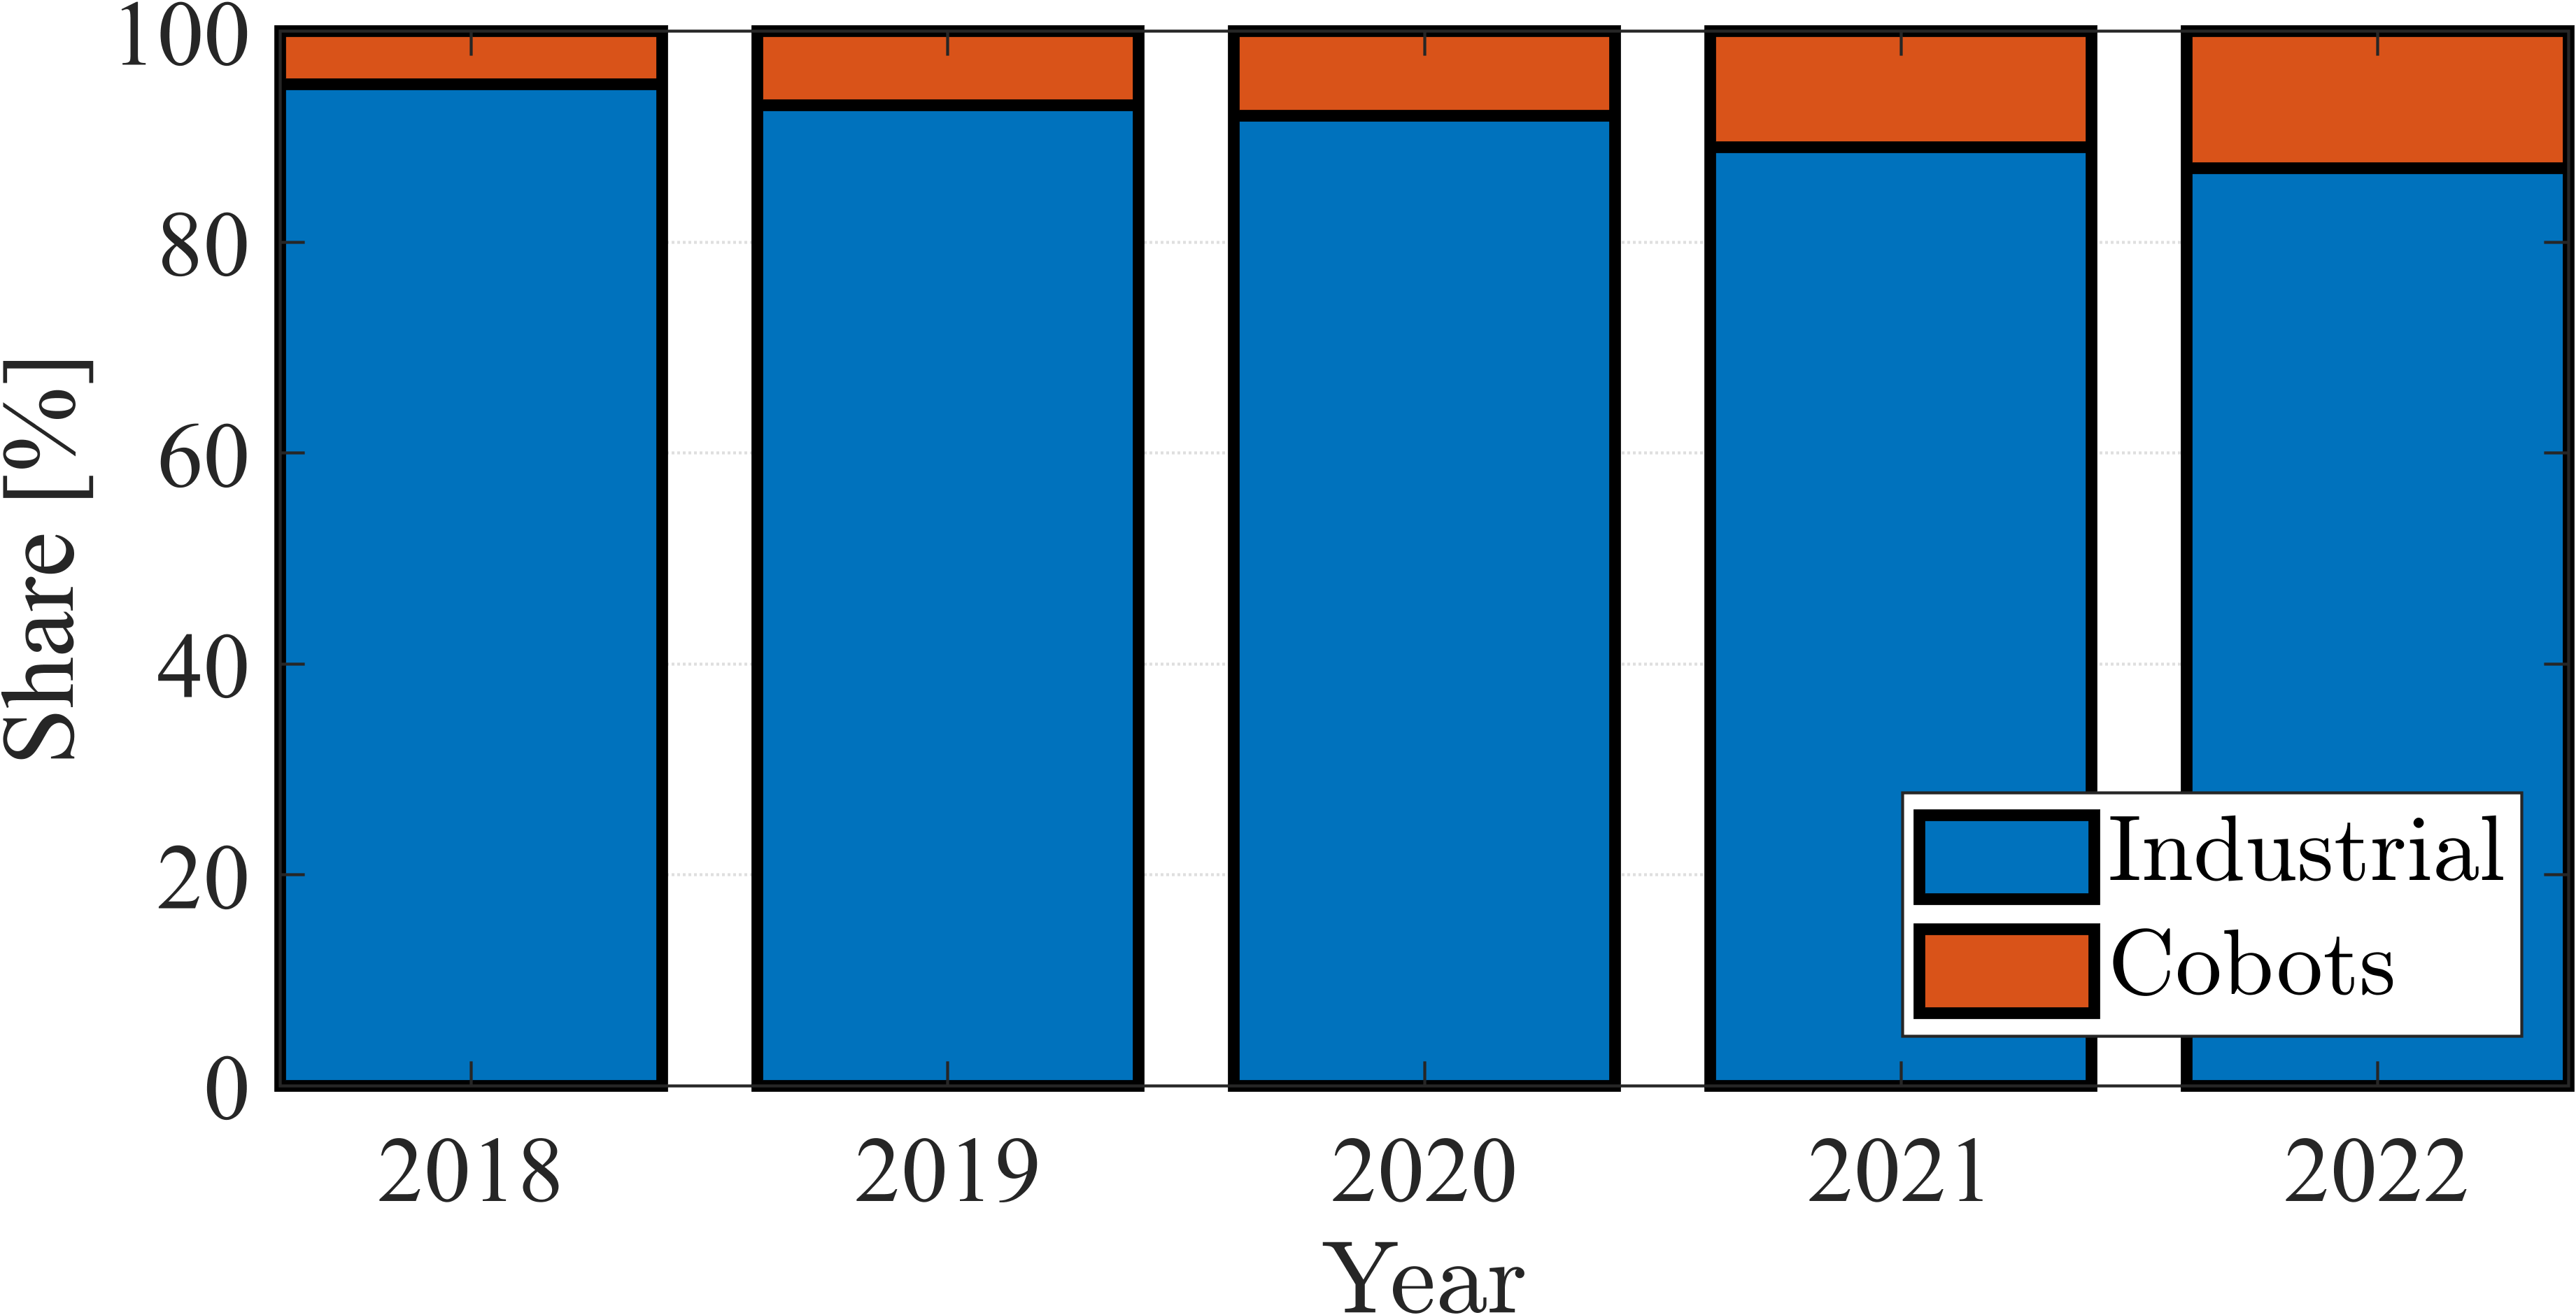
\includegraphics[width= 0.45\textwidth]{fig/share_industrial_and_cobots.png} 
	\caption{\textbf{Unit sales share industrial robots to cobots.} Cobots have been steadily gaining representation in the robotics market.}
	\label{fig:industrial_cobot_share}
\end{figure}
% ---

The unit sales are congruent with the the estimated operational stock of industrial (Fig.~\ref{fig:ir_stock}) robots and cobots (\ref{fig:cobot_stock}).
% ---
\begin{figure*}[t!]
	\centering
	\hspace*{\fill}
	\begin{subfigure}[b]{0.45\textwidth}
		\subcaption{}
		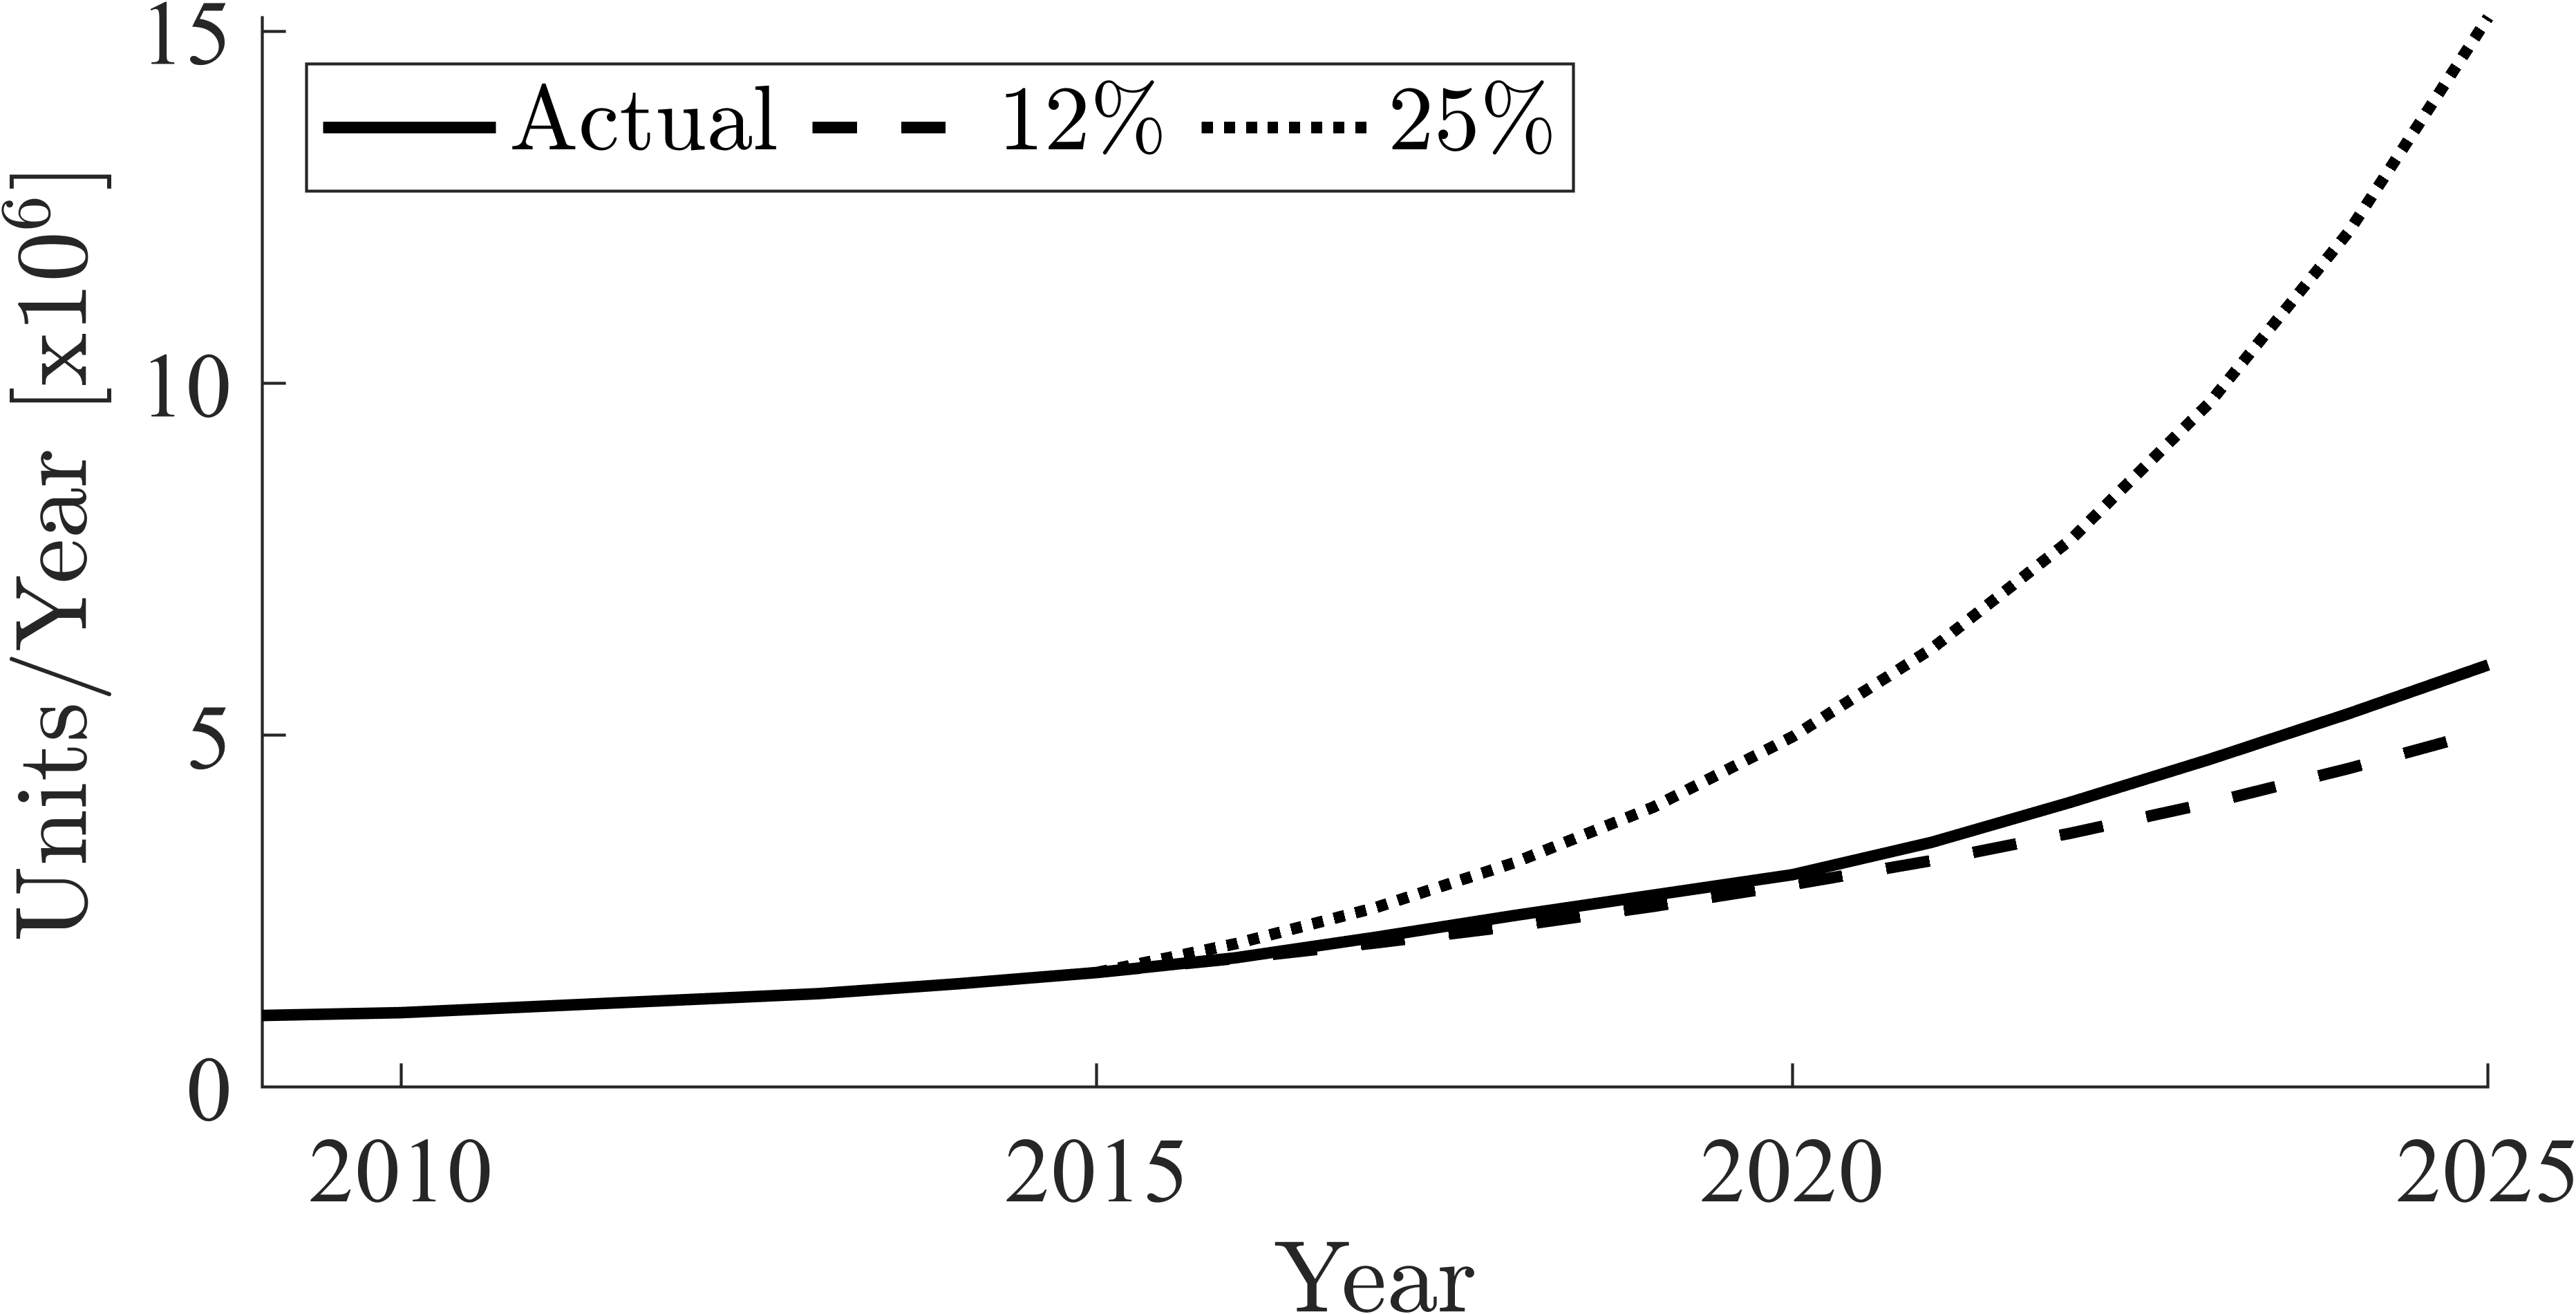
\includegraphics[width= \textwidth]{ir_units_projections.png}
		\label{fig:ir_stock}
	\end{subfigure}
	\hfill
	\begin{subfigure}[b]{0.45\textwidth}
		\subcaption{}
		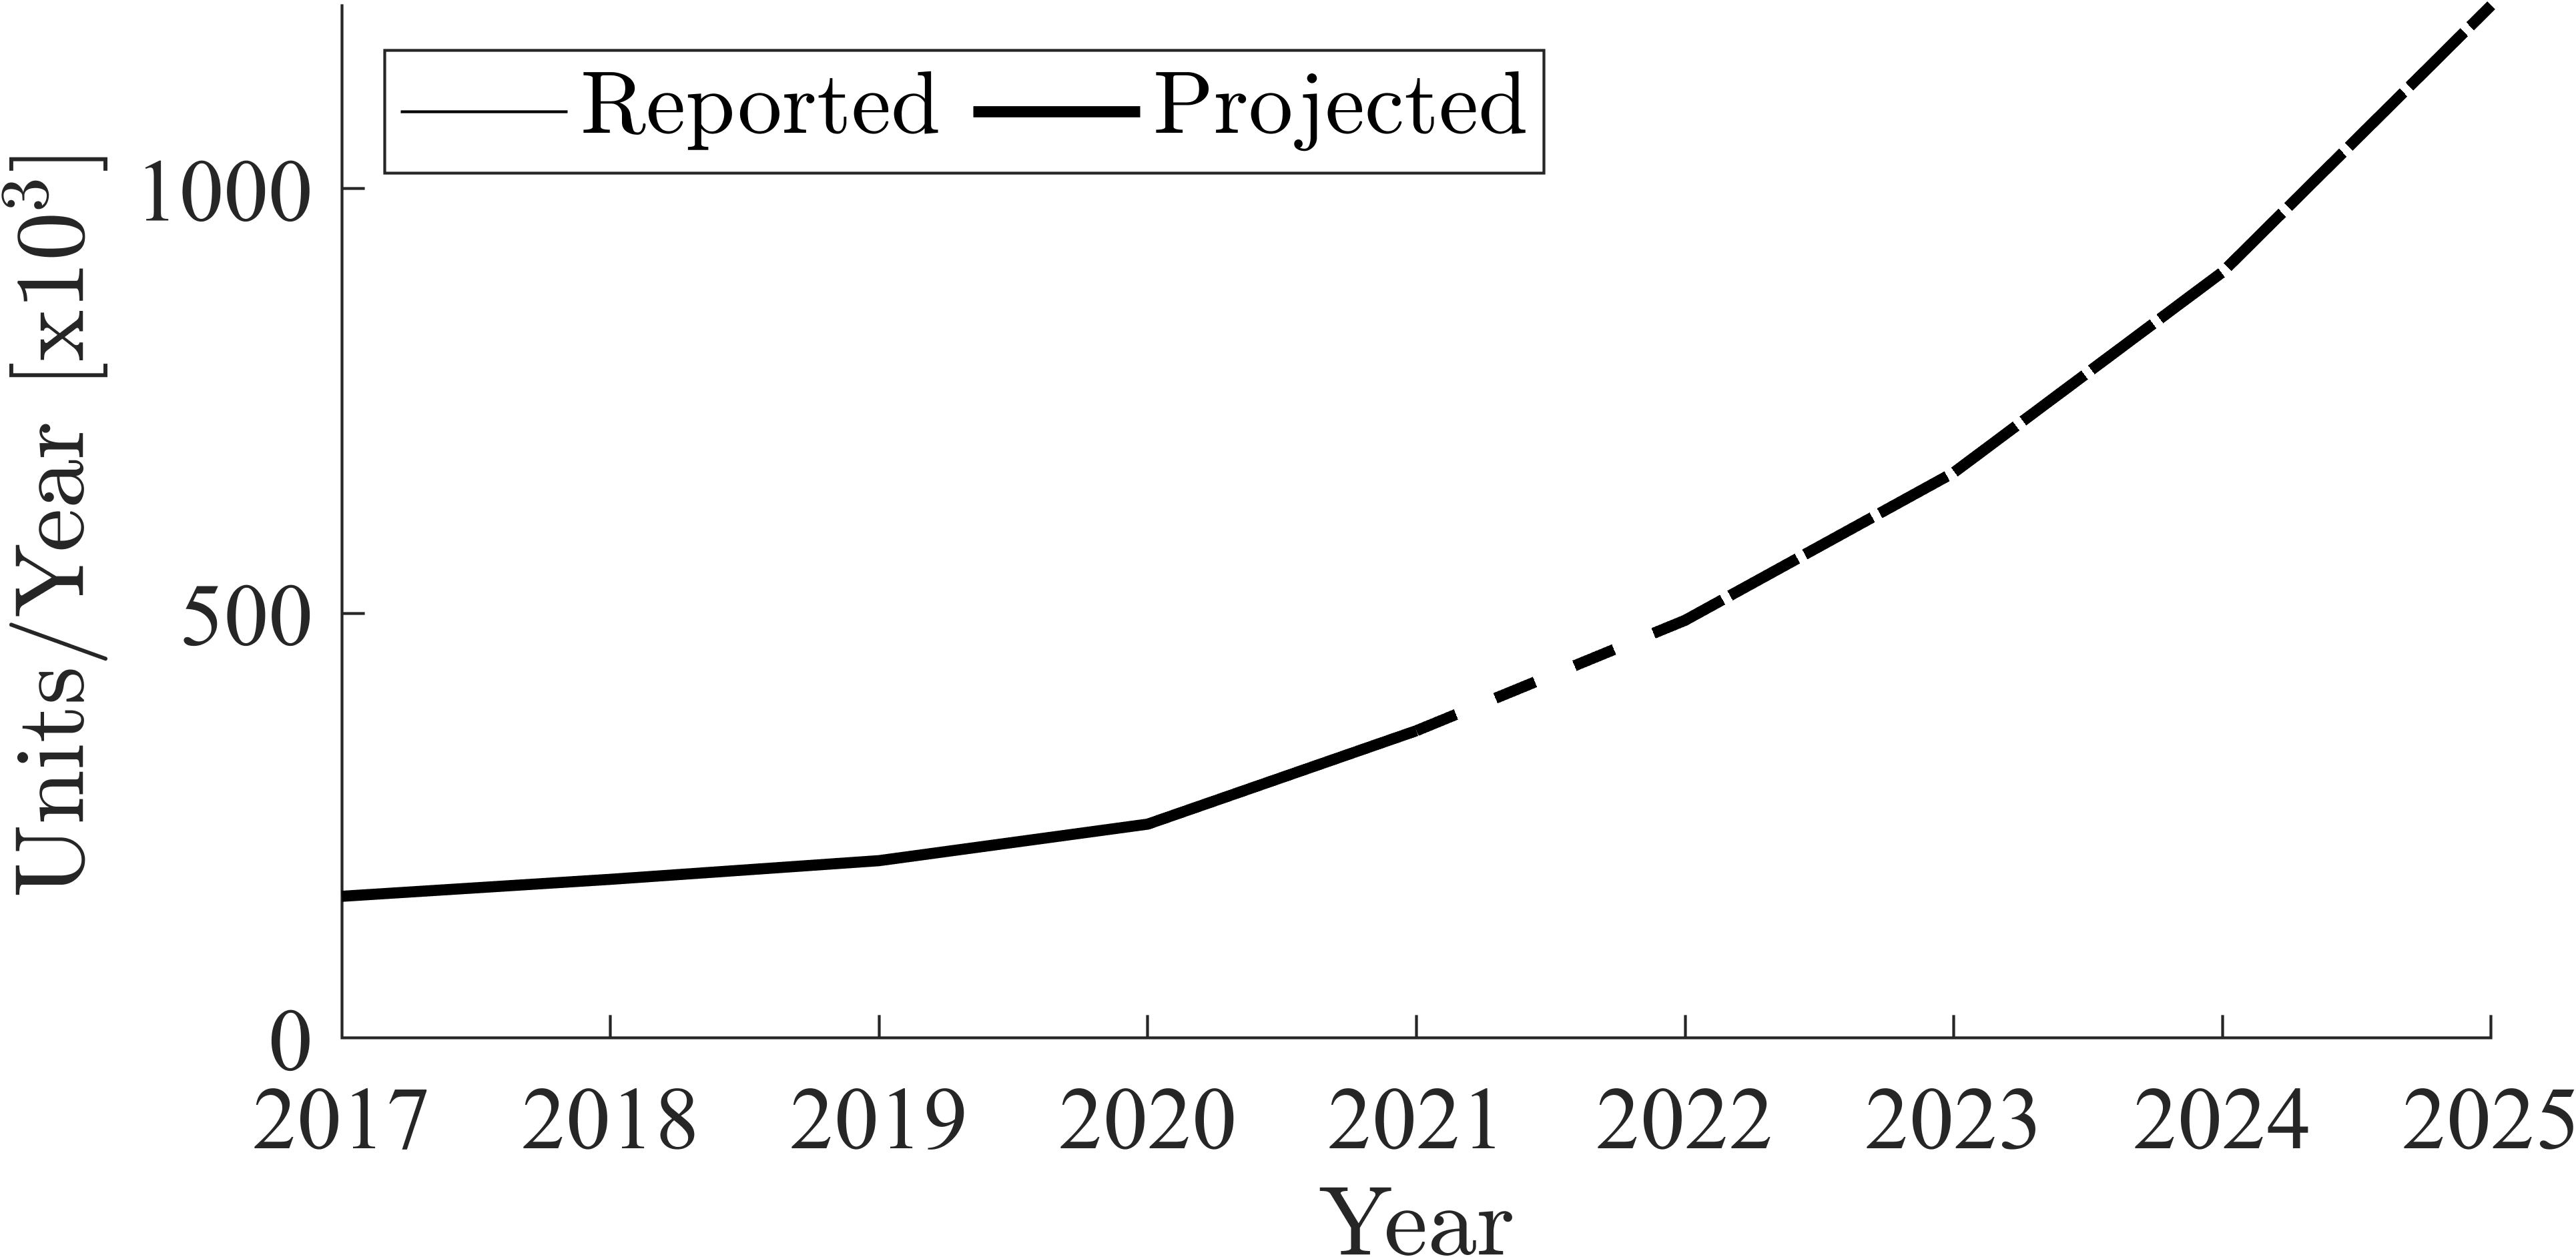
\includegraphics[width= \textwidth]{cb_units_projections.png}
		\label{fig:cobot_stock}
	\end{subfigure}
	\hspace*{\fill}	
	\caption[] {\label{fig:robot_forecasts} \textbf{Forecasts for robot operational stock.} (\subref{fig:ir_stock}) industrial robots install base forecast and (\subref{fig:cobot_stock}) cobots install base forecast.}	
\end{figure*}
% ---
% ===================================================================================================
%                                                 |                                                 |
%                                                 |                                                 |
% -------------------------------------------- SECTION ---------------------------------------------|
%                                                 |                                                 |
%                                                 |                                                 |
% ===================================================================================================
\newpage
\section{Industrial robot energy consumption support data}\label{sec:app_robot_ener_consumption}
To provide estimates of the worldwide energy consumption of industrial and collaborative robots we surveyed various sources including reports from consulting agencies and non-profit organizations, news articles and manufacturer press releases and data-sheets to determine essential data such as the operational stock and power consumption per type of robot.

\subsection{Industrial robots}
According to \cite{montaqim2015} and available press releases of different robotic companies \cite{fanuc2015, yaskawa2014, ABB2015}, the approximate distribution of the industrial robot install base per manufacturer is shown in Fig.~\ref{fig:manufacturers_pie}.
% ---
\begin{figure*}[!h]
	\centering
	\hspace*{\fill}
	\begin{subfigure}[t]{0.45\textwidth}
		\subcaption{}
		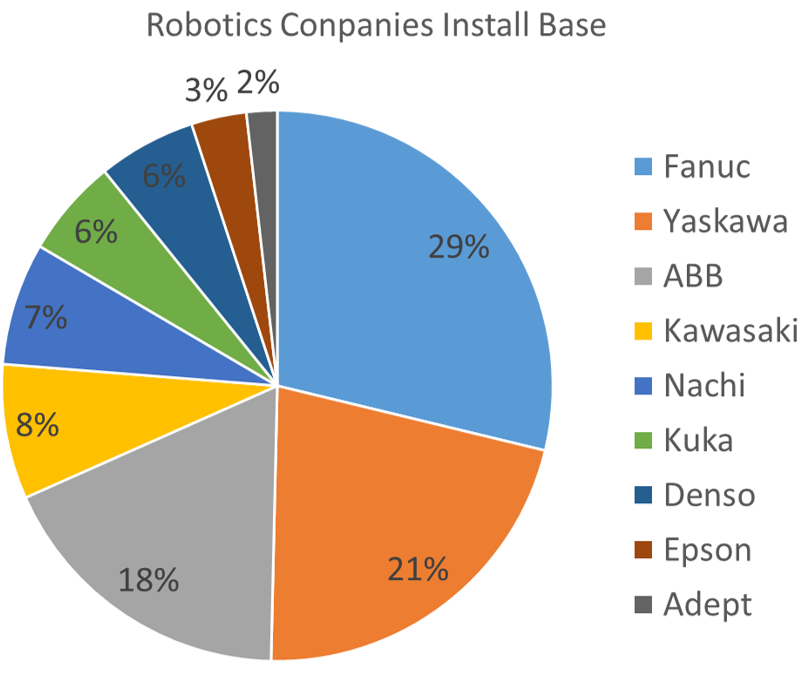
\includegraphics[width= \textwidth]{manufacturers}
		\label{fig:manufacturers_pie}
	\end{subfigure}
	\hfill
	\begin{subfigure}[t]{0.45\textwidth}
		\subcaption{}
		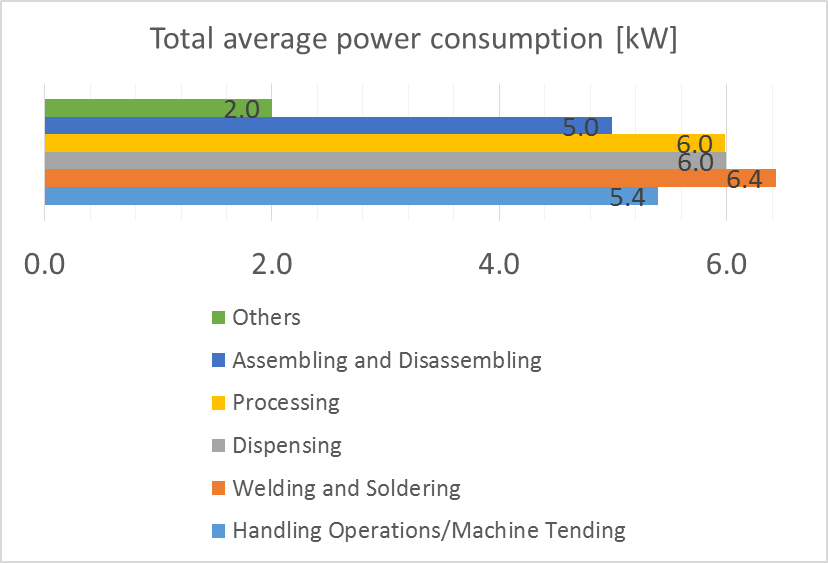
\includegraphics[width=\textwidth]{industrial_robots_average_power_per_category} \label{fig:ir_average_power}
	\end{subfigure}
	\hspace*{\fill}
	\caption[] {\label{fig:ir_statistics} \textbf{Industrial robots statistics.} (\subref{fig:manufacturers_pie}) Percentage of installed industrial robots per manufacturer and (\subref{fig:ir_average_power}) average power consumption of industrial robots per category.}
\end{figure*}
% ---

Since Fanuc, Yaskawa, and ABB make for two-thirds of the total install base of industrial robots, we took the power consumption of the robots from those manufacturers to estimate the total power consumption. After surveying the data-sheets for the different robot types in their portfolio, the average power consumption for each model was estimated. Additionally, every manufacturer classifies their robots according to one or more possible applications, which can be grouped into the application categories defined by the IFR. The average power consumption was calculated for every application using the values reported in the robot data-sheets. Finally, the power consumption for each category was computed as a weighted average based on the companies' market share percentage (assuming that 68 \% is the total number of robots)\footnote[1]{These numbers should be used with discretion since there is no available information on which are the most common installed robot models. This information may change the estimation.}. The estimated power consumption per robot application is shown in Fig.~\ref{fig:ir_average_power}. Using these numbers and the estimated operational stock of industrial robots reported in \cite{statista_ir_operational_stock} and by the International Federation of Robotics (see Fig.~\ref{fig:ir_stock}), the estimated worldwide industrial robot energy consumption was computed and shown in Fig.~\ref{fig:ir_energy}.

% ===================================================================================================
\subsection{Collaborative robots}\label{sec:app_cobot_ener_consumption}
%---
\begin{figure}[!h]
	\centering
	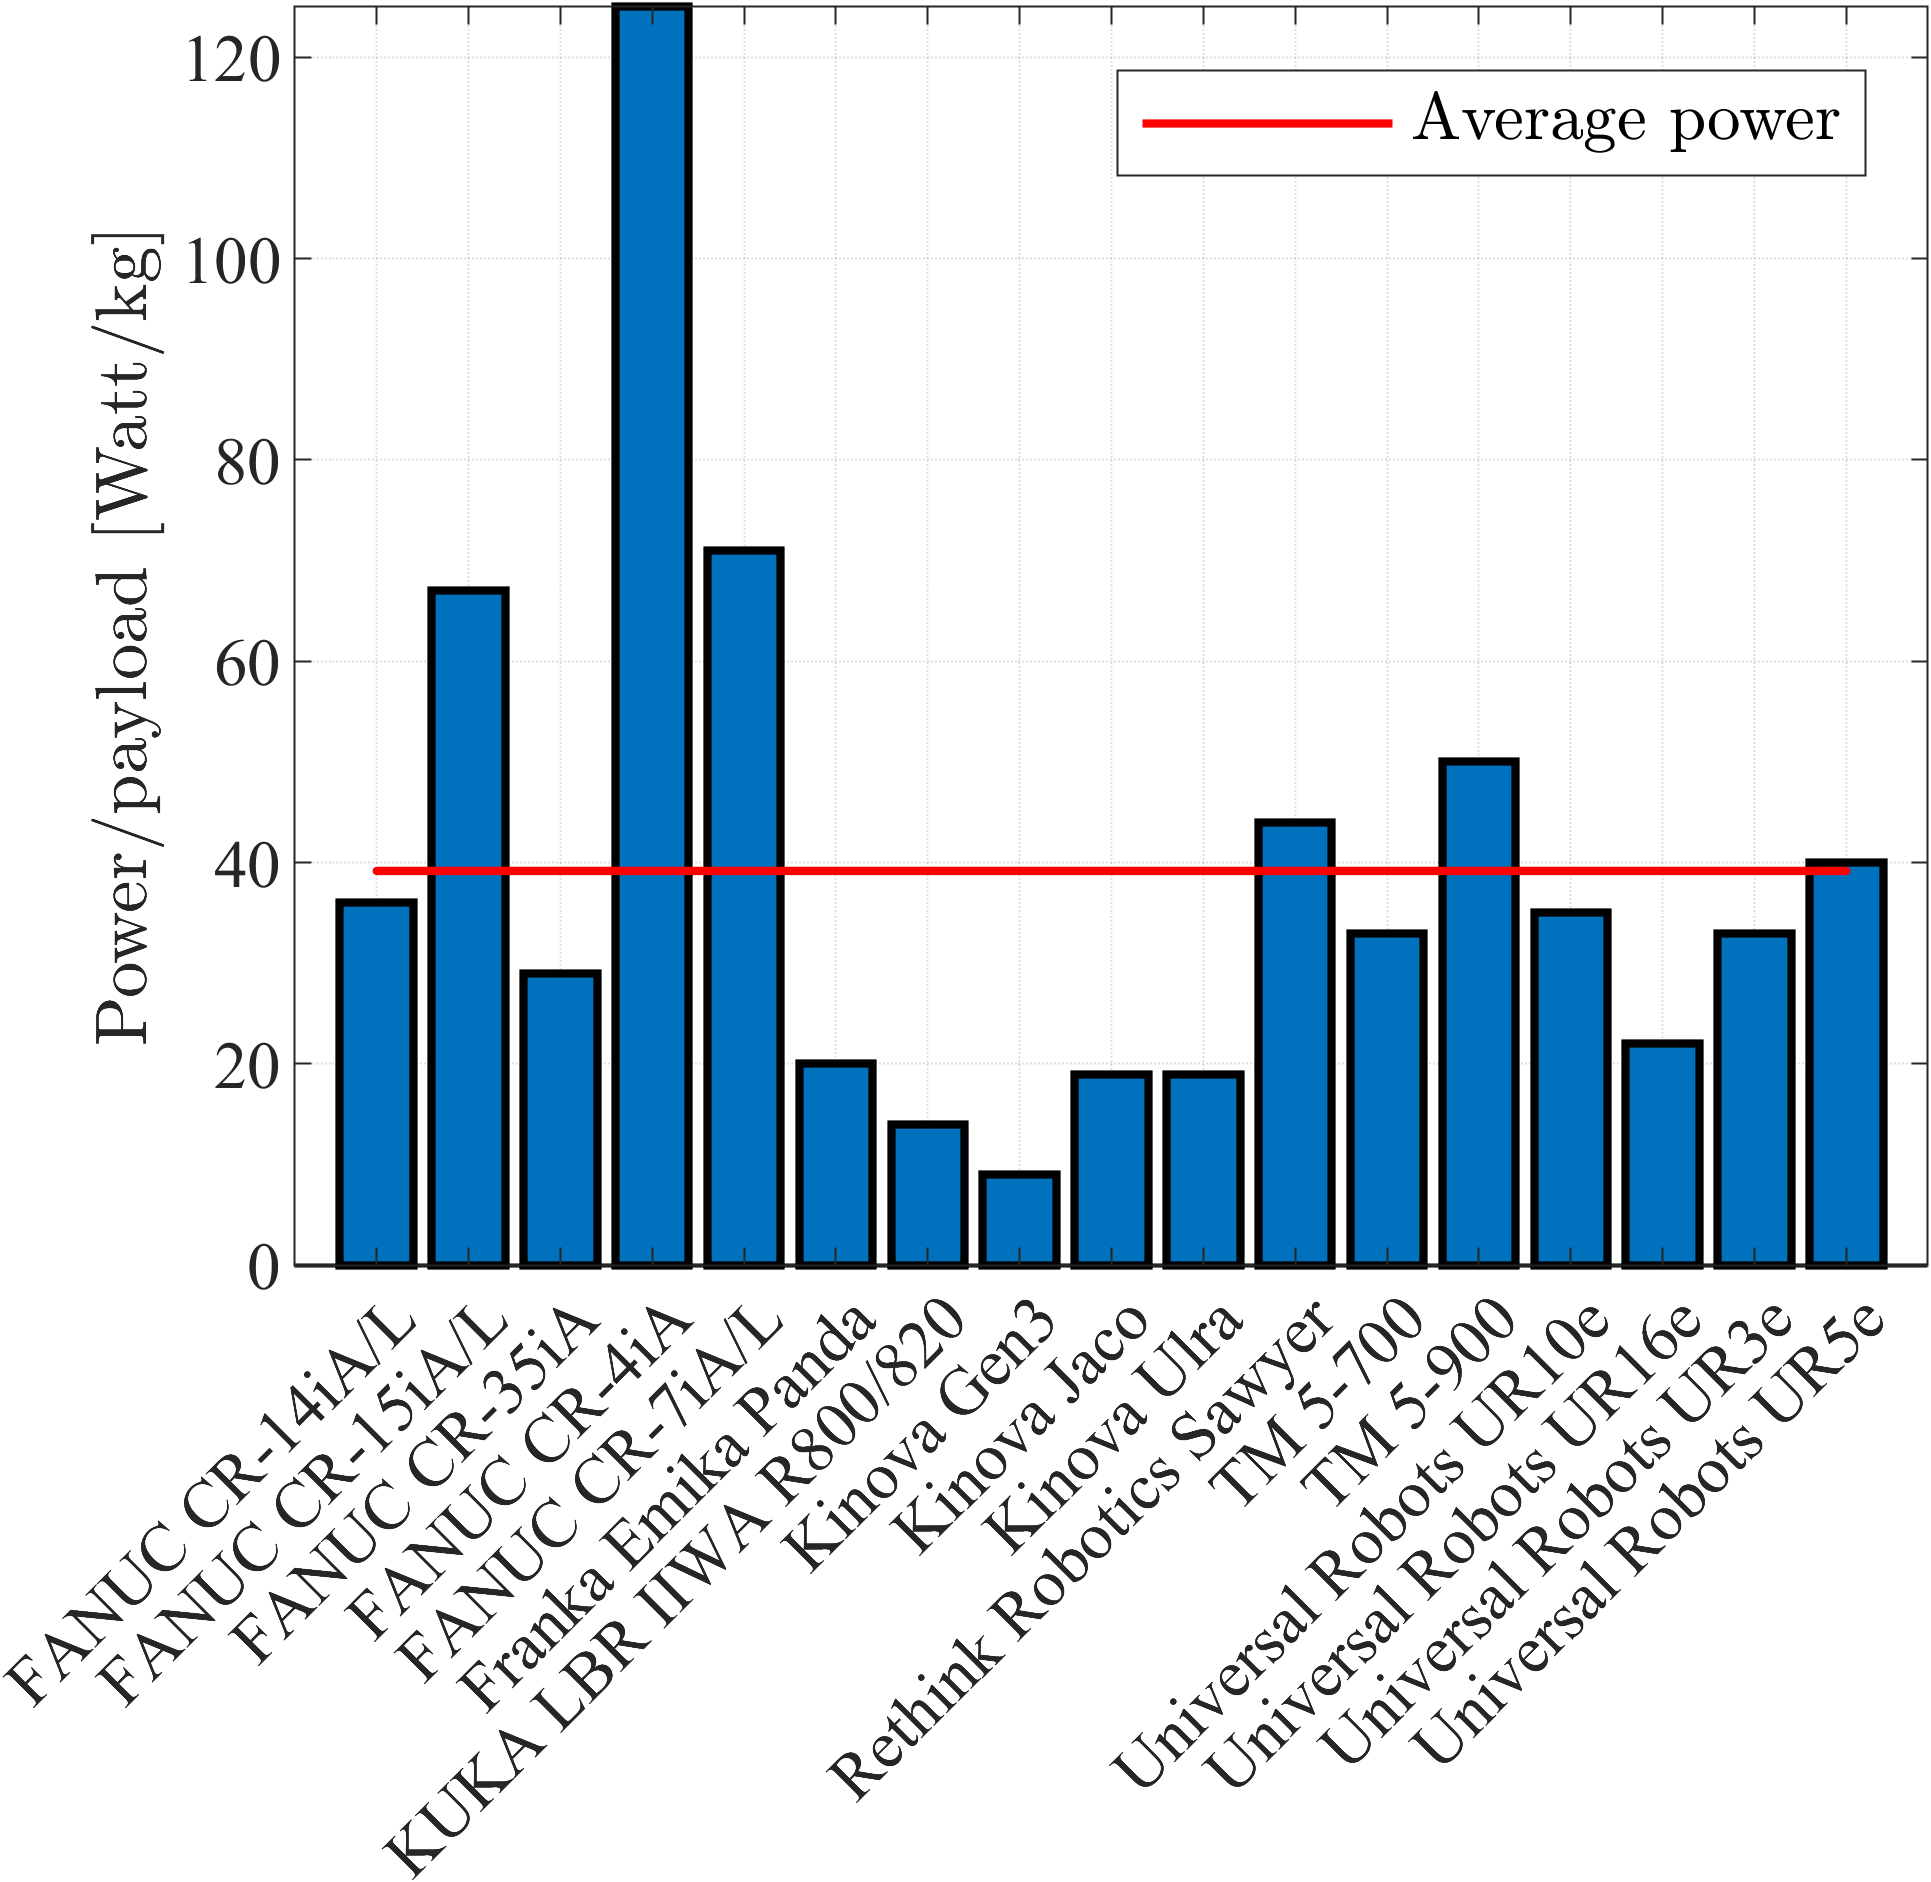
\includegraphics[width=0.45\textwidth]{cobot_watt_per_kg.png}
	\caption{\textbf{Power consumption per payload for different cobots.} The average power consumption can be estimated at around 40 W.}
	\label{fig:cobot_watt_per_kg}
\end{figure}
%---
To approximate the energy consumption of cobots we looked at the power consumption per payload of various manufacturers, see Fig.~\ref{fig:cobot_watt_per_kg} resulting in an average power consumption of approximately 40 W. Together with a typical power consumption of the robot controller of 60 W \cite{Heredia2023BreakingEnergyConsumption}, we consider a total of 100 W power demand. Similar to the industrial robots, the worldwide energy consumption was calculated assuming a 24/7 operation.



